\chapter[All the paths lead to Noto: oddness in non-scalar Hurford Disjunctions]{All the paths lead to Noto: oddness in non-scalar Hurford Disjunctions\footnotemark}\label{chap:hurford-disj}
\footnotetext{This Chapter is partly based on \citettoappear{HenotMortier2024a}, and hopefully spells out the model and arguments more extensively and explicitly. I would like to thank the audience and reviewers of SuB29 and of the 2024 BerlinBrnoVienna Workshop, in particular Alex Kalomoiros, Flavia Naehrlich, Jacopo Romoli, Benjamin Spector, and Raven Zhang, for relevant questions, datapoints and suggestions regarding earlier iterations of this project.}

This Chapter constitutes a direct follow-up of Chapter \ref{chap:redundancy}, and proposes to generalize the \textsc{Non-Redundancy} constraint introduced in that Chapter, in order to account for a range of Hurford Disjunctions \citep{Hurford1974,Marty2022}. Specifically, we will argue that the proper notion of equivalence between Qtrees that feeds \textsc{Q-Non-Redundancy} is not exactly equality (of nodes and edges) as proposed in Chapter \ref{chap:redundancy}, but instead, structural equality combined with equality between minimal strategies of inquiry -- defined in terms of optimal paths from the CS-root to verifying nodes. This will preserve the results obtained for the dataset presented in Chapter \ref{chap:redundancy}, and additionally cover the relevant Hurford cases.

\section{Introducing Huford Disjunctions}
In Chapter \ref{chap:redundancy}, we introduced a new \textsc{Non-Redundancy} constraint accounting for a problematic dataset. We showed that previous approaches to oddness either could not fully capture these data (\citenp{Katzir2014}, \citenp{Kalomoiros2024}), or could \citep{Mayr2016}, but at the cost of jeopardizing results previously obtained on other famously odd sentences. Among these famously odd sentences, are Hurford Disjunctions \citep{Hurford1974}, henceforth \textbf{HD}s, exemplified in (\ref{ex5:hd}). HDs typically feature contextually entailing disjuncts (abbreviated $p^+ \vDash p$), and are generally odd regardless of the order of the weak ($p$) vs. strong ($p^+$) disjunct.\footnote{A notable exception is when the two disjuncts are the same \textit{modulo} scalemate expressions, such as \textit{some} vs. \textit{all}; in that case, HDs may be rescued from infelicity (\citenp{Gazdar1979}; \citenp{Singh2008b}; \citenp{Fox2018}; \citenp{Ippolito2019}; \citenp{HenotMortier2023} i.a.). We do not cover these cases here, but Chapters \ref{chap:scalarity} and \ref{chap:economy} provide an overview of the challenges raised by these ``scalar'' variants, and sketch solutions based on the current framework.}

\begin{exe}
	\ex \label{ex5:hd}
	\begin{xlist}
		\ex[\#] {SuB29 will take place in Noto\footnote{Noto is located in Italy and is where the main session of SuB29 was organized.} or Italy. \hfill $\pplus\vee \p$}\label{ex5:hd-sw}
		\ex[\#] {SuB29 will take place in Italy or Noto. \hfill $\p \vee \pplus$}\label{ex5:hd-ws}
	\end{xlist}
\end{exe}

Accounting for (\ref{ex5:hd}) in an explanatory way, i.e. without simply stating that disjunctions should not feature entailing disjuncts, is challenging. First, identifying a specific, well-motivated pragmatic principle susceptible to account for (\ref{ex5:hd}) is not necessarily easy (though, Chapter \ref{chap:redundancy}, Section \ref{sec4:previous-accounts}, already foreshadowed several potential solutions). Second, pre-theoretically similar instances of oddness seem to affect expressions in which disjuncts are \textit{not} in a relation of contextual entailment. For instance, given that the Basque country encompasses Northern Central Spain and Southwestern France, saying that \textit{SuB29 will take place in the Basque country} is \textit{compatible} with saying that \textit{SuB29 will take place in France}. Yet, the sentences in (\ref{ex5:chd}) still sound quite odd \citep{Singh2008a}. We will call such expressions Compatible Hurford Disjunctions, henceforth \textbf{CHD}s.
\begin{exe}
	\ex \label{ex5:chd}
	\begin{xlist}
		\ex[\#] {SuB29 will take place in the Basque country or France. \hfill $\q\vee\p$; $\q \wedge \p \not\vDash\bot$}\label{ex5:chd-1}
		\ex[\#] {SuB29 will take place in France or in the Basque country. \hfill $\p\vee\q$; $\p \wedge \q \not\vDash\bot$}\label{ex5:chd-2}
	\end{xlist}
\end{exe} 

Relatedly, disjunctions derived from HDs by further disjoining the stronger disjunct with a proposition incompatible with the weaker disjunct, also appear quite odd \citep{Marty2022}. This is shown in (\ref{ex5:ldhd}). This is surprising essentially because, just like CHDs, such expressions feature merely compatible disjuncts. The issue seems to come from the observation that one disjunct involves a sub-expression ($p^+$) entailing the other disjunct ($p$). For this reason, these disjunctions were dubbed Long-Distance Hurford Disjunctions, henceforth \textbf{LDHD}s.

\begin{exe}
	\ex \label{ex5:ldhd}
	\begin{xlist}
		\ex[\#] {Either SuB29 will take place in Noto or Paris, or it will take place in Italy. \\ $(\pplus\vee\r)\vee\p$ \hfill $\pplus \vDash \p$; $(\pplus \vee \r)\wedge \p \not\vDash \bot$}\label{ex5:ldhd-sw}
		\ex[\#] {Either SuB29 will take place in Italy, or it will take place in Noto or Paris. \\ $\p\vee(\pplus\vee\r)$ \hfill $\pplus \vDash \p$; $(\pplus \vee \r)\wedge \p \not\vDash \bot$ }\label{ex5:ldhd-ws}
	\end{xlist}
\end{exe}


The rest of this Chapter proposes an account of these data, and is organized as follows. Section \ref{sec5:previous-accounts} reviews four existing accounts of pragmatic oddness, and shows that they can only partially account for the data presented in this introduction. Section \ref{sec5:q-non-redundancy} presents \textsc{Q-Non-Redundancy}, as defined in Chapter \ref{chap:redundancy}, shows that it is also insufficient in its current form, and proposes to update it in a ``conservative'' way, based on a new notion of equivalence between Qtrees. Section \ref{sec5:hd-account} shows that this newly defined constraint captures both HDs and LDHDs, and additionally discusses how the Qtree model in fact captures CHDs, independently of \textsc{Q-Non-Redundancy}. Section \ref{sec5:discussion} discusses a few conceptual and empirical implications of this analysis, and in particular compares it to previous \textsc{Redundancy}-based and QuD-tree-based accounts of HDs. Section \ref{sec5:ccl} concludes this Chapter.\\

We now proceed to reviewing why some of the data presented in this introduction are problematic for previous accounts of oddness (excluding the new QuD-driven approach introduced in Chapter \ref{chap:redundancy}). We will follow the same structure as in Chapter \ref{chap:redundancy}, Section \ref{sec4:previous-accounts}.

\section{Previous accounts of oddness, and their shortcomings}\label{sec5:previous-accounts}

The Section presents four existing accounts of oddness already covered in Chapter \ref{chap:redundancy}: \textsc{Global Non-Redundancy}, \textsc{Local Non-Redundancy}, \textsc{Super-Redundancy}, and \textsc{Non-Triviality}.\footnote{This Section relies extensively on \citeauthor{Marty2022}'s overview paper \citep{Marty2022}.} We show that all accounts straightforwardly capture HDs, but struggle accounting for CHDs. Some, but not all approaches, manage to capture the case of LDHDs.

\subsection{Global Non-Redundancy}

This approach builds on the idea that sentences featuring unnecessary verbosity should be deemed odd. This is cashed out in (\ref{ex4:global-non-redundancy}) (repeated from Chapter \ref{chap:redundancy}). Roughly, (\ref{ex4:global-non-redundancy}) states that, if two sentences are contextually equivalent, then the simpler one should be preferred, and the more complex one should be deviant. Simplicity is understood as structural, following \citet{Katzir2007} -- see (\ref{ex4:structural-complexity}), repeated below. We dub the principle in (\ref{ex4:global-non-redundancy}) \textsc{Global Non-Redundancy}, because contextual equivalence and simplicity are evaluated at the level of the entire sentence, and not locally.\footnote{A local variant of this principle will be investigated in the next Section.}

\begin{exe}
	\exr{ex4:global-non-redundancy} {\textsc{\textbf{Global Non-Redundancy}} \citep{Meyer2013,Mayr2016}. A sentence $S$ cannot be used in context $c$ if there is a sentence $S'$ s.t. $S'$ is a simplification of $S$ and $S' \equiv_c S$.}
	\exr{ex4:structural-complexity} {\textit{Structural simplicity \citep{Katzir2007}.} $S'$ is a simplification of $S$ if $S'$ can be derived from $S$ by replacing nodes in $S$ with their subconstituents.}
\end{exe}


(\ref{ex4:global-non-redundancy}) correctly predicts HDs to be deviant in both orders, because they are contextually equivalent to their weaker disjunct ($p^+\vee p \equiv p\vee p^+ \equiv p$).
However, it predicts CHDs and LDHDs to be fine. This is proved in (\ref{ex4:global-non-redundancy-chd}) and (\ref{ex4:global-non-redundancy-ldhd}) respectively. The issue seems to be that (\ref{ex4:global-non-redundancy}) is too ``global'' and thus not sensitive to the internal organization of the disjuncts. This is especially obvious in the case of LDHDs, whereby infelicity seems to arise from the logical relation between a ``high'', weak disjunct, and a ``low'', strong disjunct embedded within an inner disjunction.

\begin{exe}
	\ex {(\ref{ex4:global-non-redundancy}) predicts CHDs to be fine.\\
	Let \p, \q{} be s.t. $\p\wedge\q\not\vDash \bot$ (compatible), $\p\not\vDash \q$ and $\q\not\vDash \p$ (non-entailing in any direction).\\
	If $\p \vee\q \equiv \p$, then we would have $\q \vDash \p\vee\q \equiv \p$; contradiction.\\
	If $\p \vee\q \equiv \q$, then we would have $\p \vDash \p\vee\q \equiv \q$; contradiction.\\
	So $\p \vee\q \not\equiv \p$ and $\p \vee\q \not\equiv \q$.}\label{ex4:global-non-redundancy-chd}
	\ex {(\ref{ex4:global-non-redundancy}) predicts LDHDs to be fine.\\
	Let \p, \pplus and \r{} be s.t. $\pplus \vDash \p$ (``long-distance'' entailment), and $\p\wedge\r \vDash \bot$.\\
	We define \q{} as $\pplus \vee\r$.\\
	Then, \p, \q{} are s.t. $\p\wedge\q\not\vDash \bot$ (compatible), $\p\not\vDash \q$ and $\q\not\vDash \p$ (non-entailing in any direction).\\
	Therefore $\p \vee\q \not\vDash \p$ and $\p \vee\q \not\vDash \q$, as per proof (\ref{ex4:global-non-redundancy-chd}).\\
	Therefore $\p \vee (\pplus \vee \r) \not\vDash \p$ and $\p \vee(\pplus \vee \r) \not\vDash \pplus \vee \r$. }\label{ex4:global-non-redundancy-ldhd}
\end{exe}


\subsection{Local Non-Redundancy}
\citet{Katzir2014} propose a local implementation of \textsc{Global Non-Redundancy}, stating that the semantic computation evaluates, at
certain nodes, whether the composition principle that applies there is non-vacuous. This gives rise to the principle in (\ref{ex4:local-non-redundancy}).

\begin{exe}
	\exr{ex4:local-non-redundancy} {\textsc{\textbf{Local Non-Redundancy}} \citep{Katzir2014}. $S$ is deviant if $S$ contains $\gamma$ s.t. $\llbracket \gamma \rrbracket = \llbracket O(\alpha, \beta) \rrbracket \equiv_c \llbracket\zeta \rrbracket, \ \zeta \in \lbrace \alpha, \beta\rbrace$.}
\end{exe}

Just like \textsc{Global Non-Redundancy}, (\ref{ex4:local-non-redundancy}) correctly predicts HDs to be deviant in both orders, because they are contextually equivalent to their weaker disjunct ($p$). But it also incorrectly predicts CHDs to be fine, for the same reason as \textsc{Global Non-Redundancy}; see proof (\ref{ex4:global-non-redundancy-chd}). The same incorrect prediction hold for LDHDs, as shown in (\ref{ex5:local-non-redundancy-ldhd}).

\begin{exe}
	\ex {(\ref{ex4:local-non-redundancy}) predicts LDHDs to be fine.\\
		Let \p, \pplus and \r{} be s.t. $\pplus \vDash \p$ (``long-distance'' entailment), and $\p\vee\r \vDash \bot$.\\
		Evaluating the outer disjunction: $\p \vee (\pplus \vee \r) \not\vDash \p$ and $\p \vee(\pplus \vee \r) \not\vDash \pplus \vee \r$ (see proof (\ref{ex4:global-non-redundancy-ldhd})). Not locally redundant.\\
		Evaluating the inner disjunction: given that $\pplus \vDash \p$ and $\p\wedge\r \vDash \bot$, $\pplus\wedge\r \vDash \bot$ (i.e. the two disjuncts of the inner disjunction are incompatible). Therefore, $\pplus \vee \r \not \equiv \pplus$ and $\pplus \vee \r \not \equiv \r$. Not locally redundant. }\label{ex5:local-non-redundancy-ldhd}
\end{exe}

Even if \text{Local Non-Redundancy} was designed to be more ``local'',  it still cannot capture the ``long-distance'' logical dependency between $p$ and $p^+$ in LDHDs. The case of CHDs also remains problematic, due to their apparent ``opacity'': structurally, CHDs amount to one single disjunction, and as such, cannot be better captured by \textsc{Local Non-Redundancy} (as compared to \textsc{Global Redundancy}).


\subsection{Super-Redundancy}
%HDs feel redundant; while HCs sound locally irrelevant.
%Talk about repairs: the fact the repairs are differnt suggets the violation stems from a different source.

\citet{Kalomoiros2024}, elaborating on \citet{Katzir2014}'s view, introduces \textsc{Super-Redundancy}. Roughly, a sentence $S$ is super-redundant if it features a binary operation taking a constituent $C$ as argument, and moreover there is no way of strengthening $C$ to $C^+$ that would make the resulting sentence $S^+$ non-redundant (i.e., non-equivalent to its counterpart where $C^+$ got deleted).

\begin{exe}
	\exr{ex4:sr} {\textsc{\textbf{Super-Redundancy}} \citep{Kalomoiros2024}. A sentence $S$ is infelicitous if it contains $C \ast C'$ or $C' \ast C$, with $\ast$ a binary operation, s.t. $(S)^-_C$ is defined and for all $D$, $(S)^-_C \equiv S_{Str(C, D)}$. In this definition:
		\begin{itemize}
			\item $(S)^-_C$ refers to $S$ where $C$ got deleted;
			\item  $Str(C, D)$ refers to a strengthening of $C$ with $D$, defined inductively and whose key property is that it commutes with negation ($Str(\neg\alpha, D) = \neg (Str(\alpha, D))$), as well as with binary operators ($Str(O(\alpha, \beta), D) = O(Str(\alpha, D), Str(\beta, D))$);
			\item $S_{Str(C, D)}$ refers to $S$ where $C$ is replaced by $Str(C, D)$.
	\end{itemize}}
\end{exe}


Interestingly, this principle predicts both HDs and LDHDs to be degraded (see (\ref{ex5:hd-sr})\footnote{Proof adapted from the original paper \citep{Kalomoiros2024}.} and (\ref{ex5:ldhd-sr})). Thus, it constitutes an improvement over \textsc{Global/Local Non-Redundancy}.



\begin{exe}
	\ex {HDs are Super Redundant (SR).\\
	We show (\ref{ex5:hd-sw})=$\pplus\vee\p$ and (\ref{ex5:hd-ws})=$\p\vee\pplus$ are SR.\\
			In either case, take C = \pplus.\\
			We then have (\ref{ex5:hd-sw})$^-_C$ = (\ref{ex5:hd-ws})$^-_C$ = $\p$\\
			$\forall D. \ (\textref{ex5:hd-sw})_{Str(C, D)} = (\textref{ex5:hd-ws})_{Str(C, D)} =  (\pplus \wedge D) \vee \p$\\
			\phantom{$\forall D. \ (\textref{ex5:hd-sw})_{Str(C, D)} = (\textref{ex5:hd-ws})_{Str(C, D)}$} $\equiv (\pplus \vee \p) \wedge (D \vee \p)$\\
			\phantom{$\forall D. \ (\textref{ex5:hd-sw})_{Str(C, D)} = (\textref{ex5:hd-ws})_{Str(C, D)}$} $\equiv \p \wedge (D \vee \p)$\\
			\phantom{$\forall D. \ (\textref{ex5:hd-sw})_{Str(C, D)} = (\textref{ex5:hd-ws})_{Str(C, D)}$} $\equiv (\p \wedge D) \vee \p$\\
			\phantom{$\forall D. \ (\textref{ex5:hd-sw})_{Str(C, D)} = (\textref{ex5:hd-ws})_{Str(C, D)}$} $\equiv \p = (\textref{ex5:hd-sw})^-_C = (\textref{ex5:hd-ws})^-_C$ 
		}\label{ex5:hd-sr}
	\ex {LDHDs are Super Redundant (SR).\\
		We show (\ref{ex5:ldhd-sw})=$(\pplus\vee\r)\vee\p$ and (\ref{ex5:ldhd-ws})=$\p\vee(\pplus\vee\r)$ are SR.\\
		In either case, take C = \pplus.\\
		We then have (\ref{ex5:ldhd-sw})$^-_C$ = (\ref{ex5:ldhd-ws})$^-_C$ = $\p\vee\r$\\
		$\forall D. \ (\textref{ex5:ldhd-sw})_{Str(C, D)} = (\textref{ex5:ldhd-ws})_{Str(C, D)} =  ((\pplus \wedge D)\vee \r) \vee \p$\\
		\phantom{$\forall D. \ (\textref{ex5:ldhd-sw})_{Str(C, D)} = (\textref{ex5:ldhd-ws})_{Str(C, D)}$} $\equiv (\p \vee \r) \vee (\pplus \wedge D)$\\
		\phantom{$\forall D. \ (\textref{ex5:ldhd-sw})_{Str(C, D)} = (\textref{ex5:ldhd-ws})_{Str(C, D)}$} $\equiv (\p \vee \r \vee \pplus) \wedge (\p \vee \r \vee D)$\\
		\phantom{$\forall D. \ (\textref{ex5:ldhd-sw})_{Str(C, D)} = (\textref{ex5:ldhd-ws})_{Str(C, D)}$} $\equiv (\p \vee \r) \wedge (\p \vee \r \vee D)$\\
		\phantom{$\forall D. \ (\textref{ex5:ldhd-sw})_{Str(C, D)} = (\textref{ex5:ldhd-ws})_{Str(C, D)}$} $\equiv (\p \vee \r) \vee (\bot\wedge D)$\\
		\phantom{$\forall D. \ (\textref{ex5:ldhd-sw})_{Str(C, D)} = (\textref{ex5:ldhd-ws})_{Str(C, D)}$} $\equiv (\p \vee \r) \vee \bot$\\
		\phantom{$\forall D. \ (\textref{ex5:ldhd-sw})_{Str(C, D)} = (\textref{ex5:ldhd-ws})_{Str(C, D)}$} $\equiv \p \vee \r = (\textref{ex5:ldhd-sw})^-_C = (\textref{ex5:ldhd-ws})^-_C$\\
	}\label{ex5:ldhd-sr}
\end{exe}

However, this account still cannot capture the case of CHDs, again due to their structural ``opacity''. This is shown in (\ref{ex5:chd-sr}).

\begin{exe}
		\ex {CHDs are not Super Redundant (SR).\\
		We show (\ref{ex5:chd-1})=$\q \vee \p$ and (\ref{ex5:chd-2})=$\p \vee \q$ are not SR.\\
		Take C = \p.\\
		We then have  (\ref{ex5:chd-1})$^-_C$ = (\ref{ex5:chd-2})$^-_C$ = \q.\\
		Take $D=\top$.\\
		$(\textref{ex5:chd-1})_{Str(C, D)} = (\textref{ex5:chd-2})_{Str(C, D)} =  (\p \wedge D) \vee \q$\\
		\phantom{$(\textref{ex5:chd-1})_{Str(C, D)} = (\textref{ex5:chd-2})_{Str(C, D)}$} $\equiv (\p \wedge \top) \vee \q$\\
		\phantom{$(\textref{ex5:chd-1})_{Str(C, D)} = (\textref{ex5:chd-2})_{Str(C, D)}$}  $\equiv \p \vee \q$\\
		\phantom{$(\textref{ex5:chd-1})_{Str(C, D)} = (\textref{ex5:chd-2})_{Str(C, D)}$} $\not\equiv \q = (\textref{ex5:chd-1})^-_C = (\textref{ex5:chd-2})^-_C$.\\
		Same proof if C = \p, swapping the roles of \p{} and \q.\\
	}\label{ex5:chd-sr}
\end{exe}

Solving the puzzle of CHDs most likely requires us to say something \textit{explanatory} about compatible disjuncts, going beyond their intensional semantics. The Chapter will suggest that our QuD framework can essentially get CHDs ``for free'', based on how the concept of granularity gets incorporated in Qtrees, and on how disjunctive Qtrees get computed.


\subsection{Non-Triviality}\label{sec5:non-triviality}
A different line of work (\citeauthor{Mayr2016}, \citeyear{Mayr2016} i.a.), building on the notion of Local Contexts \citep{Schlenker2009}, associates oddness with triviality in the sense of \citep{Stalnaker1999}. This view is summarized in (\ref{ex4:non-triviality}), repeated from Chapter \ref{chap:redundancy}.

\begin{exe}
	\exr{ex4:non-triviality} {\textsc{\textbf{Non-Triviality}} \citep{Mayr2016}. A sentence $S$ cannot be used in a context $c$ if some part $\pi$ of $S$ is entailed or contradicted by the Local Context of $\pi$ in $c$ (abbreviated LC($\pi$, $c$)).}
	\ex {\textit{Local Context. } The Local Context of an expression $\pi$ in a sentence $S$ is the smallest domain that one may restrict attention to when assessing E without jeopardizing the truth conditions of $S$. Let $c$ be the global context of $S$. The above definition derives the following facts for disjunctions and conditionals:
		\begin{xlist}
			\ex {If $S$ is a conditional of the form $\Phi \rightarrow \Psi$, LC($\Phi$, $c$) = $c$ and LC($\Psi$, $c$) = $c\cap\Phi$.}
			\ex {If $S$ is a disjunction of the form $\Phi \vee \Psi$, and LCs are assumed to be computed incrementally (left-to-right), LC($\Phi$, $c$) = $c$ and LC($\Psi$, $c$) = $c\cap\neg\Phi$}
			\ex {If $S$ is a disjunction of the form $\Phi \vee \Psi$, and LCs are assumed to be computed symmetrically (left-to-right and right-to-left), LC($\Phi$, $c$) = $c\cap\neg\Psi$ and LC($\Psi$, $c$) = $c\cap\neg\Phi$.}
	\end{xlist}}
\end{exe}

Chapter \ref{chap:redundancy} briefly mentioned the tension between HDs and the dataset presented in that Chapter. Let us briefly review the arguments here.


Assuming LCs are computed \textit{symmetrically} for disjunctions (see (\ref{ex4:lc-disj-sym})), (\ref{ex4:non-triviality}) predicts the right pattern for HDs. This is shown in (\ref{ex5:hurford-non-triviality-sym}).

\begin{exe}
	\ex {Assuming symmetric Local Contexts, we show HDs of the form \pplus{} $\vee$ \p{} or \p{} $\vee$ \pplus{} are correctly predicted to be infelicitous.\\
		Take $\pi = $ \pplus{} ((\ref{ex5:hd-sw})'s 1st disjunct / (\ref{ex5:hd-ws})'s 2nd disjunct).\\
		LC($\pi$, $c$) = $c\cap(\neg\p)$, contradiction.\\
	}\label{ex5:hurford-non-triviality-sym}
\end{exe}

Assuming instead that LCs are computed \textit{asymmetrically} for disjunctions (see (\ref{ex4:lc-disj-incr})), (\ref{ex4:non-triviality}) incorrectly predicts strong-to-weak HDs to be fine. This is shown in (\ref{ex5:hurford-non-triviality-asym}).

\begin{exe}
	\ex {Assuming asymmetric Local Contexts, we show Hurford Disjunctions of the form \pplus{} $\vee$ \p{} are incorrectly predicted to be felicitous.\\
		Take $\pi =$ (\ref{ex4:hd-sw})'s 1st disjunct  = \pplus.\\
		LC($\pi$, $c$) = $c$, consistent.\\
		Take $\pi =$ (\ref{ex4:hd-sw})'s 2nd disjunct  = \p.\\
		LC($\pi$, $c$) = $c\cap(\neg\pplus)$, consistent.\\
	}\label{ex5:hurford-non-triviality-asym}
\end{exe}

Therefore, accounting for HDs \textit{via} \textsc{Non-Triviality} requires symmetric Local Contexts. However, Chapter \ref{chap:redundancy} introduced data that we argued could \textit{only} be captured assuming \textit{asymmetric} Local Contexts (in particular, felicitous sentences of the form $p \vee (\neg p \rightarrow q)$).\footnote{(\ref{ex4:pv(nptq)-repeated-nt}) and (\ref{ex4:target-sentences-non-triviality-sym}), repeated from Chapter \ref{chap:redundancy} below, show that only asymmetric Local Context capture the felicity of sentences of the form $p \vee (\neg p \rightarrow q)$. This clashes with the assumptions needed to capture HDs under the \textsc{Non-Triviality} view.
\begin{exe}
	\exr{ex4:pv(nptq)-repeated-nt} {\noindent We show  (\ref{ex4:pv(nptq)-repeated})=$\p \vee (\neg \p \rightarrow \q)$ is not locally trivial.\\
		Take $\pi =$ (\ref{ex4:pv(pvq)-repeated})'s 1st disjunct  = \p. LC($\pi$, $c$) = $c$, consistent.\\
		Take $\pi =$ (\ref{ex4:pv(pvq)-repeated})'s antecedent  = $\neg$\p. LC($\pi$, $c$) = LC($\neg \p$, $c$) = $\neg$\p{} (negation of 1st disjunct), consistent. \\
		Take $\pi =$ (\ref{ex4:pv(pvq)-repeated})'s consequent  = \q. LC($\pi$, $c$) = LC($\q$, $c$) = $\neg$\p{} (negation of 1st disjunct / antecedent), consistent. 
	}
	\exr{ex4:target-sentences-non-triviality-sym} {Assuming symmetric Local Contexts, we show (\ref{ex4:pv(nptq)-repeated})=$\p \vee (\neg \p \rightarrow \q)$ is locally trivial.\\
		Take $\pi =$ (\ref{ex4:pv(pvq)-repeated})'s 1st disjunct  = \p.\\
		LC($\pi$, $c$) = $c\cap\neg(\neg\p\rightarrow\q)$ = $c\cap(\neg\p\wedge\neg\q)$, contradiction with \p.
	}
\end{exe}
} In other words, (\ref{ex4:non-triviality}) cannot capture the data presented in Chapter \ref{chap:redundancy} along with HDs, based on unified underlying assumptions.\\

Turning to LDHDs and CHDs, \textsc{Non-Triviality} can account for LDHDs assuming symmetric Local Contexts (see (\ref{ex5:ldhd-non-triviality-sym})). 

\begin{exe}
	\ex {Assuming symmetric Local Contexts, we show LDHDs of the form $(\pplus \vee\r)\vee \p$ or $\p\vee(\pplus \vee\r)$ are correctly predicted to be infelicitous.\\
		Take $\pi = $ \pplus{} ((\ref{ex5:ldhd-sw})'s / (\ref{ex5:ldhd-ws})'s 1st inner disjunct).\\
		LC($\pi$, $c$) = $c\cap(\neg\p)$, contradiction.\\
	}\label{ex5:ldhd-non-triviality-sym}
\end{exe}

However, just like   previously introduced \textsc{Redundancy}-based accounts, \textsc{Non-Triviality} cannot deal with the case of CHDs. This is shown in (\ref{ex5:chd-non-triviality-sym}) assuming symmetric Local Contexts. It is easy to see that assuming asymmetric Local Contexts does not help resolve the issue.

\begin{exe}
	\ex {Assuming symmetric Local Contexts, we show CHDs of the form $\q \vee \p$ or $\p \vee \q$ (with \p{} and \q{} logically compatible but non-entailing) are incorrectly predicted to be felicitous.\\
		Take $\pi =$ \q{} ((\ref{ex5:chd-1})'s 1st disjunct / (\ref{ex5:chd-2})'s 2nd disjunct).\\
		LC($\pi$, $c$) = $c\cap\p$, consistent.\\
		Take $\pi =$ \p{} ((\ref{ex5:chd-1})'s 2nd disjunct / (\ref{ex5:chd-2})'s 1st disjunct).\\
		LC($\pi$, $c$) = $c\cap\q$, consistent.\\
	}\label{ex5:chd-non-triviality-sym}
\end{exe}




We have just reviewed four prominent accounts of pragmatic oddness, and showed that, even if then can all capture basic HDs, they cannot capture CHDs. Some, but not all accounts, managed to capture LDHDs. This calls for another approach to these Hurford Sentences, that would capture their oddness despite structural opacity (in the case of CHDs), or structural ``distance'' between occurrences of redundant material (in the case of LDHDs). The next Section explores the predictions of our QuD-driven \textsc{Non-Redundancy} constraint introduced in Chapter \ref{chap:redundancy} -- dubbed \textsc{Q-Non-Redundancy}. We show that these predictions appear unsatisfying at first blush, but suggest a possible update of \textsc{Q-Non-Redundancy} that could cover the cases at stake, while crucially retaining the good results obtained for the data in Chapter \ref{chap:redundancy}.



%\begin{exe}
%	\ex[\#] {Jo either does\textcolor{blue}{n't study in France}, or \textcolor{orange}{not in Europe} or in \textcolor{green}{Paris}.	\hfill \textbf{\textcolor{blue}{q}} $\vee$ (\textcolor{orange}{\textbf{q}$^+$} $\vee$ \r)\\
%			with: \textbf{\textcolor{blue}{q}} := $\neg$\pplus; \textcolor{orange}{\textbf{q}$^+$} := $\neg$\p }
%\end{exe}
%
%We think that both (\ref{ex5:ldhd-pos}) and (\ref{ex5:ldhd-neg}) are degraded -- which is in itself interesting because SR predicts (\ref{ex5:ldhd-neg}) to be fine.

 


\section[Q-Non-Redundancy]{Q-Non-Redundancy, and its shortcomings}\label{sec5:q-non-redundancy}

\subsection{Summary of the current account}

In Chapter \ref{chap:redundancy}, we introduced a new \textsc{Non-Redundancy} constraint on LF-Qtree pairs, and showed that this constraint, unlike \textsc{Global/Local/Super Redundancy}, could capture a challenging dataset based on logical variations of $p \vee p \vee q$. This constraint, dubbed \textsc{Q-Non-Redundancy} and repeated in (\ref{ex4:Q-Non-Redundancy}), can be summarized as follows. If a Qtree $Q$ is evoked by a sentence $S$ and also by one of the sentence's formal simplifications $S'$, then $Q$ is deemed \textsc{Q-Redundant} given $S$. This definition is based on the concept of structural simplicity, repeated in (\ref{ex4:structural-complexity}) below.

\begin{exe}
	\exr{ex4:Q-Non-Redundancy} {\textsc{\textbf{Q-Non-Redundancy}} (to be revised). Let $X$ be a LF and let $Qtrees(X)$ be the set of Qtrees evoked by $X$. For any $T \in Qtrees(X)$, $T$ is deemed \textsc{Q-Redundant} given $X$ (and thus, odd given $X$) iff there exists a formal simplification of $X$, $X'$, and $T' \in Qtrees(X')$, such that $T=T'$.}
	\exr{ex4:q-equivalence} {\textsc{\textbf{Qtree equality}}. $T = T'$ iff $T$ and $T'$ have same structure and same verifying nodes.}
	\exr{ex4:structural-complexity} {\textsc{\textbf{Structural simplicity}} \citep{Katzir2007}. $S'$ is a simplification of $S$ if $S'$ can be derived from $S$ by replacing nodes in $S$ with their subconstituents.}
\end{exe}

Additionally, a sentence that is compatible with no Qtree is deemed odd -- see (\ref{ex2:oddness-sentence}).

\begin{exe}
	\exr{ex2:oddness-sentence} {\textsc{\textbf{Oddness of a sentence}}. A sentence $S$ is odd if any Qtree $T$ it evokes is odd given $S$.}
\end{exe}


\subsection{An issue with the current account}

\textsc{Q-Non-Redundancy}, as defined in (\ref{ex4:Q-Non-Redundancy}), unfortunately cannot even account for HDs. To see this, let us compute the Qtrees compatible with $S_p = $ \textit{SuB29 will take place in Italy}, $S_{p^+} = $ \textit{SuB29 will take place in Noto}, as well the Qtree(s) compatible with their two possible disjunctions (\ref{ex5:hd-sw}) and (\ref{ex5:hd-ws}).

Chapter \ref{chap:accommodating-quds} extensively discussed how to derive Qtrees from simplex sentences like $S_p$ and $S_{p^+}$. Here, it is enough to say that such sentences may evoke three kinds of Qtrees: ``polar'' ones, splitting the Context Set (henceforth \textbf{CS}) into $p$ and $\neg p$ worlds; ``\textit{wh}'' ones, splitting the CS according to the Hamblin partition generated by same-granularity alternatives to the prejacent; and ``\textit{wh}-articulated'' ones, whereby each layer corresponds to a Hamblin partition of increasing granularity from the top down, the last layer matching the granularity of the prejacent. In each case, leaves entailed by the prejacent are \setlength{\fboxsep}{1pt}\fbox{flagged} as ``verifying'', and as such keep track of at-issue content. In this Chapter, we will only consider two levels of granularity for $S_p$ and $S_{p^+}$: by-city and by-country. This gives rise to the Qtrees in Figure \ref{fig5:qtrees-noto} (for $S_{p^+}$) and Figure \ref{fig5:qtrees-italy} (for $S_{p}$). 

\begin{figure}[H]
	\centering
	\begin{subfigure}[b]{.2\linewidth}
		\centering
		\scalebox{1}{
			\begin{forest}
				[CS [\fbox{\textcolor{orange}{Noto}}] [$\neg$\textcolor{orange}{Noto}]]
			\end{forest}
		}\caption[]{``Polar''.}\label{fig5:qtree-noto-polar}
	\end{subfigure}\hfill
	\begin{subfigure}[b]{.37\linewidth}
		\centering
		\scalebox{1}{
			\begin{forest}
				[CS [\fbox{\textcolor{orange}{Noto}}] [\textcolor{orange}{Rome}][\textcolor{orange}{Paris}][\textcolor{orange}{...}]]
			\end{forest}
		}\caption[]{``\textit{Wh}''.}\label{fig5:qtree-noto-wh}
	\end{subfigure}\hfill
	\begin{subfigure}[b]{.37\linewidth}
		\centering
		\scalebox{1}{
			\begin{forest}
				[CS[\textcolor{blue}{Italy} [\fbox{\textcolor{orange}{Noto}}] [\textcolor{orange}{Rome}] [\textcolor{orange}{...}]] [\textcolor{blue}{France}[\textcolor{orange}{Paris}][\textcolor{orange}{...}]] [\textcolor{blue}{...}]]
			\end{forest}
		}\caption[]{``\textit{Wh}-articulated''.}\label{fig5:qtree-noto-tiered}
	\end{subfigure}
	\caption[]{Qtrees evoked by $S_{\pplus}$ = \textit{SuB29 will take place in Noto}.}\label{fig5:qtrees-noto}
\end{figure}
\begin{figure}[H]
	\centering

	\begin{subfigure}[b]{.45\linewidth}
		\centering
		\scalebox{1}{
			\begin{forest}
				[CS [\fbox{\textcolor{blue}{Italy}}] [$\neg$\textcolor{blue}{Italy}]]
			\end{forest}
		}\caption[]{``Polar''.}\label{fig5:qtree-italy-polar}
	\end{subfigure}\hfill
	\begin{subfigure}[b]{.45\linewidth}
		\centering
		\scalebox{1}{
			\begin{forest}
				[CS [\fbox{\textcolor{blue}{Italy}}] [\textcolor{blue}{France}][\textcolor{blue}{...}]]
			\end{forest}
		}\caption[]{``\textit{Wh}''.}\label{fig5:qtree-italy-wh}
	\end{subfigure}
	\caption[]{Qtrees evoked by $S_{\p}$ = \textit{SuB29 will take place in Italy}.}\label{fig5:qtrees-italy}
\end{figure}

Looking at Figures \ref{fig5:qtrees-noto} and \ref{fig5:qtrees-italy}, we can observe that the Qtrees in \ref{fig5:qtree-noto-polar}, \ref{fig5:qtree-noto-wh}, and \ref{fig5:qtree-italy-polar}, introduce orthogonal partitionings of the CS, as defined in (\ref{ex2:orthogonality}), repeated below. 

\begin{exe}
	\exr{ex2:orthogonality} {\textsc{\textbf{Orthogonal partitions}}. Let $T = (\mathcal{N}, \mathcal{E}, R)$ and $T' = (\mathcal{N}', \mathcal{E}, R)$ be two depth-$1$ Qtrees sharing the same root $R$ (equivalently, two partitions of the same CS). $T$ and $T'$ are orthogonal iff they involves two nodes that are strictly overlapping, i.e. $\exists (N, N') \in \mathcal{N}\times\mathcal{N'}. \ N \cap N' \neq \emptyset \wedge N \neq N'$. $T$ and $T'$ are orthogonal iff $T$ and $T'$ exhibit a partition clash.}
\end{exe}


By contrast, Figures \ref{fig5:qtree-noto-tiered} and \ref{fig5:qtree-italy-wh}, introduce consistent partitionings: Figure \ref{fig5:qtree-noto-tiered} can be in fact be seen as a refinement of Figure \ref{fig5:qtree-italy-wh}, as per (\ref{ex2:qtree-refinement}), repeated below.

\begin{exe}
	\exr{ex2:qtree-refinement} {\textsc{\textbf{Qtree refinement}}. Let $T$ and $T'$ be Qtrees. $T$ is a refinement of $T'$ (or: $T$ is finer-grained than $T'$), iff $T'$ can be obtained from $T$ by removing a subset $\mathcal{T}$ of $T$'s subtrees, s.t., if $\mathcal{T}$ contains a subtree rooted in $N$, then, for each node $N'$ that is a sibling of $N$ in $T$, the subtree of $T$ rooted in $N'$, is also in $\mathcal{T}$.}
\end{exe}

%	In our case, this predicts that two sentences evoking different levels of granularity (e.g., city-level vs. country level) can in principle be disjoined by picking Qtrees $T$ and $T'$ for resp. the finer-grained and coarser-grained disjunct, s.t. $T$, constitutes a refinement of $T'$ as per (\ref{ex6:refinement-def}).

%Here it is enough to say that disjunction returns all the well-formed unions of Qtrees evoked by its individual disjuncts. A union of two Qtrees $T$ and $T'$ will be well-formed if there is no node $N$ present in both $T$ and $T'$ that introduces different partitionings in $T$ and $T'$. The set of verifying nodes attached to the two disjoined Qtrees, are also unioned. A disjunctive Qtree is thus a Qtree adressing the questions evoked by each disjunct \textit{in parallel}, making both disjuncts at issue. It is a symmetric operation: the order of the disjuncts does not influence the output. 
	
Now turning to the HDs (\ref{ex5:hd-sw}) and (\ref{ex5:hd-ws}), the Qtree(s) evoked by the disjunction of $S_p$ and $S_{p^+}$, correspond to the well-formed union(s) of Qtrees evoked by $S_p$ and $S_{p^+}$. Verifying nodes are also unioned. Chapter \ref{chap:accommodating-quds} in fact showed that depth-$1$ Qtrees corresponding to orthogonal partitions, are never properly disjoinable, in the sense that the output of the Qtree union operation, cannot be a Qtree. Relatedly, this Chapter showed, using analog sentences, that the HDs (\ref{ex5:hd-sw}) and (\ref{ex5:hd-ws}) are only compatible with one well-formed Qtree, namely, the Qtree obtained by unioning Figure \ref{fig5:qtree-noto-tiered} (for $S_{p^+}$), and Figure \ref{fig5:qtree-italy-wh} (for $S_{p}$), which, as we have just argued, stand in a refinement relation. The result of this union, depicted in Figure \ref{fig5:qtree-noto-or-italy}, is evoked by both (\ref{ex5:hd-sw}) and (\ref{ex5:hd-ws}). It is structurally equal to the input Qtree for $p^+$ (Figure \ref{fig5:qtree-noto-tiered}), but flags two verifying nodes (\textit{Italy} and \textit{Noto}) instead of one.

\begin{figure}[H]
	\centering
	\scalebox{1}{
		\begin{forest}
			[CS[\fbox{\textcolor{blue}{Italy}} [\fbox{\textcolor{orange}{Noto}}] [\textcolor{orange}{Rome}][\textcolor{orange}{...}]] [\textcolor{blue}{France}[\textcolor{orange}{Paris}][\textcolor{orange}{...}]] [\textcolor{blue}{...}]]
		\end{forest}
	}
	\caption[]{Only Qtree evoked by (\ref{ex5:hd-sw}) = $S_{\pplus} \vee S_{\p}$ or (\ref{ex5:hd-ws}) = $S_{\p} \vee S_{\pplus}$.}\label{fig5:qtree-noto-or-italy}
\end{figure}

Is this Qtree ill-formed, according to previously introduced constraints? First, this Qtree flags a non-empty set of nodes. Therefore, it does not trigger the \textsc{Empty Labeling} condition, repeated below.

\begin{exe}
	\exr{ex2:vacuous-flagging} {\textsc{\textbf{Empty labeling}}. If a sentence $S$ evokes a Qtree $T$ but does not flag any node as verifying in $T$, then $T$ is deemed odd given $S$.}
\end{exe}

Is the Qtree in Figure \ref{fig5:qtree-noto-or-italy} \textsc{Q-Redundant} given (\ref{ex5:hd-sw})/(\ref{ex5:hd-ws}) then? Our current definition of \textsc{Q-Non-Redundancy}, calls for structural equality \textit{and} equality of verifying nodes, between the Qtree in Figure \ref{fig5:qtree-noto-or-italy}, and some Qtree evoked by a simplification of (\ref{ex5:hd-sw})/(\ref{ex5:hd-ws}), i.e. $S_p$ or $S_{p^+}$. Such Qtrees are precisely the ones depicted in Figures \ref{fig5:qtrees-noto} and \ref{fig5:qtrees-italy}. Are any of these Qtrees equal to the one in Figure \ref{fig5:qtree-noto-or-italy}, in terms of structure and verifying nodes?

Focusing on verifying nodes, it is quite easy to see that none of the Qtrees in Figure \ref{fig5:qtrees-noto} or \ref{fig5:qtrees-italy}, have same verifying nodes as the Qtree in Figure \ref{fig5:qtree-noto-or-italy}. This is because the Qtree in Figure \ref{fig5:qtree-noto-or-italy}, has two verifying nodes (\textit{Noto}, and \textit{Italy}), while those in Figures Figure \ref{fig5:qtrees-noto} or \ref{fig5:qtrees-italy}, only have one (\textit{either} \textit{Noto}, or \textit{Italy}). Therefore, the HDs (\ref{ex5:hd-sw})/(\ref{ex5:hd-ws}) evoke a Qtree that is not equal to \textit{any} Qtree evoked by simplifications of (\ref{ex5:hd-sw})/(\ref{ex5:hd-ws}), and, as a result, this Qtree cannot be deemed \textsc{Q-Redundant} given (\ref{ex5:hd-sw})/(\ref{ex5:hd-ws}).

This implies that there is no constraint in our current toolkit that predicts the HDs in (\ref{ex5:hd-sw})/(\ref{ex5:hd-ws}) to be odd: they remain compatible with one well-formed Qtree, namely the one in Figure \ref{fig5:qtree-noto-or-italy}. Moreover, it can be shown that \textsc{Q-Non-Redundancy} struggles with LDHDs, essentially for the same reason. We will further discuss this case, along with the case of CHDs, after proposing an update to \textsc{Q-Non-Redundancy}. But let us first confirm that updating \textsc{Q-Non-Redundancy} is the way to go -- as opposed to updating other core components of the current machinery.


\subsection{Should we update the rule for disjunctive Qtrees?}
We have just seen that our current version of \textsc{Q-Non-Redundancy} could not even capture HDs. The natural conclusion is that \textsc{Q-Non-Redundancy} should be updated to cover such cases. However, a perhaps less intuitive solution, would be to keep \textsc{Q-Non-Redundancy} as it is, and instead, update the rule used to build disjunctive Qtrees. The hope is that updating such a rule would bock the derivation of well-formed Qtree for HDs. This Section shows that choosing this path is probably a bad idea, and that updating \textsc{Q-Non-Redundancy} should be the preferred way to go. It also better delineates what \textsc{Q-Non-Redundancy} should \textit{rule-in}.

The argument is based on the disjunctive sentences in (\ref{ex5:diff-gran-disj}), featuring incompatible disjuncts.\footnote{I thank Amir Anvari for mentioning these examples to me.} Such sentences appear close to HDs, in the sense that they are disjunctive, and also feature disjuncts of different granularities: \textit{Noto} is a city-level alternative, while \textit{France} and \textit{not Italy} are country-level. Yet, both (\ref{ex5:noto-or-not-italy}) and (\ref{ex5:noto-or-france}) sound significantly more acceptable than HDs. This suggests that such disjunctions give rise to well-formed Qtrees. We can in turn conclude that the process deriving disjunctive Qtrees should not in principle ban Qtrees evoking different levels of specificity (i.e. Qtrees standing in a refinement relation), from being unioned together.

\begin{exe}
	\ex \label{ex5:diff-gran-disj}
	\begin{xlist}
		\ex {SuB29 will take place in Noto or will not take place in Italy. \hfill $\pplus\vee \neg\p$}\label{ex5:noto-or-not-italy}
		\ex {SuB29 will take place in Noto or in France. \hfill $\pplus\vee\textbf{\textcolor{blue}{q}}$}\label{ex5:noto-or-france}
	\end{xlist}
\end{exe}

To get a better intuition as to how \textsc{Q-Non-Redundancy} should be updated, let us see what disjunctive Qtrees for (\ref{ex5:noto-or-not-italy}) and (\ref{ex5:noto-or-france}) look like. Because (\ref{ex5:noto-or-not-italy}) and (\ref{ex5:noto-or-france}) are felicitous, at least some of these Qtrees should be well-formed -- providing information about what \textsc{Q-Non-Redundancy} should \textit{rule-in}. Qtrees for $S_q$ = \textit{SuB29 will take place in France}, and $\neg S_p$ = \textit{SuB29 will not take place in Italy}, are given in Figures \ref{fig5:qtrees-france} and \ref{fig5:qtrees-not-italy}, respectively. Such Qtrees are similar to those evoked by $S_p$ = \textit{SuB29 will take place in Italy}, except that, in the case of \textit{France}, the roles of the \textit{Italy} and \textit{France} nodes are swapped; and, in the case of \textit{not Italy}, verifying nodes are flipped by negation.

\begin{figure}[H]
	\centering
	\begin{subfigure}[b]{.45\linewidth}
		\centering
		\scalebox{1}{
			\begin{forest}
				[CS [\fbox{\textcolor{blue}{France}}] [$\neg$\textcolor{blue}{France}]]
			\end{forest}
		}\caption[]{``Polar''.}\label{fig5:qtree-france-polar}
	\end{subfigure}\hfill
	\begin{subfigure}[b]{.45\linewidth}
		\centering
		\scalebox{1}{
			\begin{forest}
				[CS [{\textcolor{blue}{Italy}}] [\fbox{\textcolor{blue}{France}}][\textcolor{blue}{...}]]
			\end{forest}
		}\caption[]{``\textit{Wh}''.}\label{fig5:qtree-france-wh}
	\end{subfigure}
	\caption[]{Qtrees evoked by $S_{\textbf{\textcolor{blue}{q}}}$ = \textit{SuB29 will take place in France}.}\label{fig5:qtrees-france}
\end{figure}

\begin{figure}[H]
	\centering
	\begin{subfigure}[b]{.45\linewidth}
		\centering
		\scalebox{1}{
			\begin{forest}
				[CS [{\textcolor{blue}{Italy}}] [\fbox{$\neg$\textcolor{blue}{Italy}}]]
			\end{forest}
		}\caption[]{``Polar''.}\label{fig5:qtree-not-italy-polar}
	\end{subfigure}\hfill
	\begin{subfigure}[b]{.45\linewidth}
		\centering
		\scalebox{1}{
			\begin{forest}
				[CS [{\textcolor{blue}{Italy}}] [\fbox{\textcolor{blue}{France}}][\fbox{\textcolor{blue}{...}}]]
			\end{forest}
		}\caption[]{``\textit{Wh}''.}\label{fig5:qtree-not-italy-wh}
	\end{subfigure}
	\caption[]{Qtrees evoked by $\neg S_{\p}$ = \textit{SuB29 will not take place in Italy}.}\label{fig5:qtrees-not-italy}
\end{figure}
Such Qtrees can be disjoined with Qtrees evoked by \textit{Noto} pretty much similarly to HDs. This is done in Figure \ref{fig5:qtrees-diff-gran}.

\begin{figure}[H]
	\centering
	\begin{subfigure}[b]{.45\linewidth}
		\centering
		\scalebox{1}{
			\begin{forest}
				[CS [\textcolor{blue}{Italy}[\fbox{\textcolor{orange}{Noto}}][\textcolor{orange}{Rome}][\textcolor{orange}{...}]] [\fbox{\textcolor{blue}{France}} [\textcolor{orange}{Paris}][\textcolor{orange}{...}]]  [\fbox{\textcolor{blue}{...}}]]
		\end{forest}}
		\caption[]{Qtree evoked by (\ref{ex5:noto-or-not-italy}), resulting from (\ref{fig5:qtree-noto-tiered}) $\vee$ (\ref{fig5:qtree-not-italy-wh}).}
		\label{fig5:qtree-noto-or-not-italy}
	\end{subfigure}\hfill
	\begin{subfigure}[b]{.45\linewidth}
		\centering
		\scalebox{1}{
			\begin{forest}
				[CS [\textcolor{blue}{Italy}[\fbox{\textcolor{orange}{Noto}}][\textcolor{orange}{Rome}][\textcolor{orange}{...}]] [\fbox{\textcolor{blue}{France}} [\textcolor{orange}{Paris}][\textcolor{orange}{...}]]  [\textcolor{orange}{...}]]
		\end{forest}}
		\caption[]{Qtree evoked by (\ref{ex5:noto-or-france}), resulting from (\ref{fig5:qtree-noto-tiered}) $\vee$ (\ref{fig5:qtree-france-wh}).}
		\label{fig5:qtree-noto-or-france}
	\end{subfigure}
	\caption[]{Qtrees for felicitous disjunctions involving disjuncts with different granularities.}\label{fig5:qtrees-diff-gran}
\end{figure}


These two examples and their Qtrees suggest what the issue might be with the infelicitous HDs (\ref{ex5:hd-sw}-\ref{ex5:hd-ws}) and their Qtree in Figure \ref{fig5:qtree-noto-or-italy}: in this Qtree, the path connecting the root to the verifying node \textit{Noto}, properly contains the path connecting the root to the verifying node \textit{Italy}. Entertaining these two paths -- or strategies of inquiry -- appears suboptimal: why inquire about a country like \textit{Italy}, if one already inquires about a city like \textit{Noto}? The Qtrees in Figure \ref{fig5:qtree-noto-or-not-italy} and \ref{fig5:qtree-noto-or-france} do not exhibit similar contained paths. We will further formalize these intuitions and relate them to pragmatic competition, when updating \textsc{Q-Non-Redundancy} in the next Section.\\


This Section showed that the current way to derive disjunctive Qtrees, although it allows to generate \textit{a priori} well-formed Qtrees for HDs, turns out useful to generate Qtrees for closely related yet felicitous sentences such as (\ref{ex5:noto-or-not-italy}-\ref{ex5:noto-or-france}). This motivates an update of \textsc{Q-Non-Redundancy} ruling out HDs and ruling in (\ref{ex5:noto-or-not-italy}-\ref{ex5:noto-or-france}), as opposed to an update of the whole recipe deriving disjunctive Qtrees. We now show that updating \textsc{Q-Non-Redundancy} to capture HDs, is pretty straightforward, and moreover, can be easily shown to preserve the good results obtained in Chapter \ref{chap:redundancy} (fast forward to Section \ref{sec5:extension}).
\subsection{Updating \textsc{Q-Non-Redundancy}}

The predictions of \textsc{Q-Non-Redundancy} appear unsatisfying at first blush, but deriving Qtrees for the HDs in (\ref{ex5:hd-sw})/(\ref{ex5:hd-ws}) and their simplifications, suggests a way forward. Let us further precisify the intuition. In Figure \ref{fig5:qtree-noto-or-italy}, the two verifying nodes, \textit{Noto} and \textit{Italy}, appear on the same path originating from the CS root, and reaching the \textit{Noto}-leaf. Recall that Chapter \ref{chap:accommodating-quds}, Section \ref{sec:interpreting-qtrees}, identified paths from the CS-root to any node with ``strategies of inquiry'', i.e. sequences of conditional questions of increasing specificity. In Figure \ref{fig5:qtree-noto-or-italy}, \textit{Noto} and \textit{Italy} are thus part of the same strategy of inquiry -- the path from the CS-root to \textit{Noto}. Additionally, one can argue that the verifying status of \textit{Noto} and \textit{Italy}, gives this particular strategy of inquiry a special status, as well: it is \textit{the} strategy of inquiry that converges to at-issue nodes.

Now, let us turn to Figure \ref{fig5:qtree-noto-tiered}, the ``\textit{wh}-articulated'' Qtree evoked by $S_{p^+}$, a simplification of the HDs in (\ref{ex5:hd-sw})/(\ref{ex5:hd-ws}). As noted previously, this Qtree is almost the same as the one evoked by HDs, in Figure \ref{fig5:qtree-noto-or-italy}. The only difference is that Figure \ref{fig5:qtree-noto-tiered} only flags the \textit{Noto} node as verifying, while Figure \ref{fig5:qtree-noto-or-italy} flags both \textit{Noto} and \textit{Italy}. What about strategies of inquiry? The strategy of inquiry made at-issue by \textit{Noto} in Figure \ref{fig5:qtree-noto-tiered}, happens to be exactly the same as the strategy of inquiry made at-issue by both \textit{Noto} and \textit{Italy} in Figure \ref{fig5:qtree-noto-or-italy}. This is because, any path from the CS to both \textit{Noto} and \textit{Italy}, is a path to \textit{Noto}.

In other words, if only structure and at-issue strategies of inquiry are considered when comparing Qtrees, the Qtree in Figure \ref{fig5:qtree-noto-or-italy} (evoked by HDs), appears identical to the one in Figure \ref{fig5:qtree-noto-tiered} (evoked by a simplification of HDs). We use this observation to update \textsc{Q-Non-Redundancy}. (\ref{ex5:q-non-redundancy}) states that a Qtree evoked by a sentence is redundant if it is \textit{equivalent} (instead of \textit{equal}) to a Qtree evoked by one the sentence's formal simplifications.

\begin{exe}
	\ex {\textsc{\textbf{Q-Non-Redundancy}} (final version). Let $X$ be a LF and let $Qtrees(X)$ be the set of Qtrees evoked by $X$. For any $T \in Qtrees(X)$, $T$ is deemed \textsc{Q-Redundant} given $X$, iff there exists a formal simplification of $X$, $X'$, and $T' \in Qtrees(X')$, such that $T\equiv T'$.}\label{ex5:q-non-redundancy}
\end{exe}

(\ref{ex5:q-equivalence}) defines equivalence between Qtrees in terms of both tree structure and optimal strategies of inquiry: two Qtrees are equivalent, if their structures and optimal strategies of inquiry are the same. Optimal strategies of inquiry, are defined as the smallest set of paths from the CS-root to each existing verifying node. This is unpacked in (\ref{ex5:min-paths}).

\begin{exe}
	\ex {\textsc{\textbf{Qtree equivalence relation}}. $T$ and $T'$ are equivalent ($T \equiv T'$) iff $T$ and $T'$ have same structure and same set of minimal verifying paths.}\label{ex5:q-equivalence}
	\ex \label{ex5:min-paths}
	\begin{xlist}
		\ex {\textsc{\textbf{Verifying Paths}}. The set of verifying paths $\mathbb{P}(T)$ of a Qtree $T$ is the set of paths starting from the root of $T$, and such that each path finishes in some $N \in \mathbb{N}^+(T)$, and each $N \in \mathbb{N}^+(T)$ belongs to some path.}\label{ex5:verifying-paths}
		\ex {\textsc{\textbf{Path containment}}. Two paths $p_1$ and $p_2$ are in a containment relation ($p_1 \subseteq_{\mathbb{P}} p_2$) if $p_1$ (seen as an ordered list, i.e. a string, of nodes) is a prefix of $p_2$.}\label{ex5:path-containment}
		\ex {\textsc{\textbf{Set of minimal verifying paths}}. The set of minimal verifying paths $\mathbb{P}^*(T)$ of a Qtree $T$ is the set of minimal elements of $\mathbb{P}(T)$ w.r.t. the path containment relation.}\label{ex5:min-verifying-paths}
	\end{xlist}
\end{exe}

Figure \ref{fig5:path-containment} provides a few examples illustrating how minimal sets of verifying paths are computed. In these Figures, paths are identified by their color. Each path leads to a verifying node, whose ``box'' features the same color as the path leading to it. Figure \ref{fig5:path-containment-disjoint} illustrate the case in which the two paths at stake are entirely disjoint. As a result, the set of minimal verifying paths, is the same as the initial set of paths. Figure \ref{fig5:path-containment-included} illustrate the case in which
the two paths are in a containment relation: the orange path from the CS to A, is a prefix of the blue path from the CS to A to B. Therefore, the orange path is contained in the blue path as per (\ref{ex5:path-containment}), and the set of minimal verifying paths only contains the blue path, from the CS, to A, to B. Lastly, Figure \ref{fig5:path-containment-included} illustrates the case in which the three paths at stake exhibit some mixed overlap: the blue and orange paths both go from the CS to A, but diverge after A. Therefore, they do not stand in any kind of containment relation. The green path, is a prefix of both the blue and the orange path, and so is contained in both paths. As a result, the set of minimal verifying paths, only contains the blue and the orange paths.
\begin{figure}[H]
	\centering
	\begin{subfigure}[b]{.3\linewidth}
		\centering
		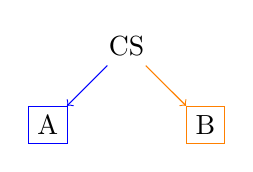
\begin{tikzpicture}
			\node[] (A) at (0, 0) {CS};
			\node[rectangle, draw=blue] (B) at (-1, -1) {A};
			\node[rectangle, draw=orange] (C) at (1, -1) {B};
			
			\draw[->, color=blue] (A) -- (B);
			\draw[->,color=orange] (A) -- (C);
		\end{tikzpicture}
		\caption[]{Fully disjoint paths.\newline$\mathbb{P} = \lbrace\textcolor{blue}{[CS;A]}, \textcolor{orange}{[CS;B]}\rbrace$\newline
			\textcolor{blue}{[CS;A]} $\not\subseteq_{\mathbb{P}}$  \textcolor{orange}{[CS;B]}\newline \textcolor{orange}{[CS;B]} $\not\subseteq_{\mathbb{P}}$ \textcolor{blue}{[CS;A]}\newline$\mathbb{P}^* = \lbrace\textcolor{blue}{[CS;A]}, \textcolor{orange}{[CS;B]}\rbrace$}\label{fig5:path-containment-disjoint}
	\end{subfigure}
	\hfill
	\begin{subfigure}[b]{.3\linewidth}
		\centering
		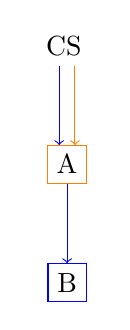
\begin{tikzpicture}
			\node[] (A1) at (0, 0) {~CS};
			\node[] (A2) at (.2, 0) {\phantom{CS}};
			\node[rectangle] (B3) at (0, -1.5) {\phantom{A}};
			\node[rectangle, draw=orange] (B1) at (0.1, -1.5) {A};
			\node[] (B2) at (.2, -1.5) {\phantom{A}};
			\node[rectangle, draw=blue] (C) at (0.1, -3) {B};
			
			\draw[->, color=blue] (A1) -- (B3);
			\draw[->, color=blue] (B1) -- (C);
			\draw[->,color=orange] (A2) -- (B2);
		\end{tikzpicture}
		\caption[]{Contained paths.\newline$\mathbb{P} = \lbrace\textcolor{blue}{[CS;A;B]}, \textcolor{orange}{[CS;A]}\rbrace$\newline
			\textcolor{orange}{[CS;A]} $\subseteq_{\mathbb{P}}$ \textcolor{blue}{[CS;A;B]}, \newline$\mathbb{P}^* = \lbrace\textcolor{blue}{[CS;A;B]}\rbrace$}\label{fig5:path-containment-included}
	\end{subfigure}
	
	\begin{subfigure}[b]{.4\linewidth}
		\centering
		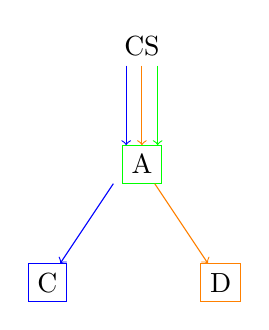
\begin{tikzpicture}
			\node[] (A1) at (0, 0) {\phantom{CS}};
			\node[] (A2) at (.2, 0) {CS};
			\node[] (A3) at (.4, 0) {\phantom{CS}};
			\node[] (B1) at (0, -1.5) {\phantom{A}};
			\node[rectangle, draw=green] (B2) at (.2, -1.5) {A};
			\node[] (B3) at (.4, -1.5) {\phantom{A}};
			\node[rectangle, draw=blue] (C1) at (-1, -3) {C};
			\node[rectangle, draw=orange] (C2) at (1.2, -3) {D};
			
			\draw[->, color=blue] (A1) -- (B1);
			\draw[->, color=blue] (B1) -- (C1);
			\draw[->, color=orange] (B2) -- (C2);
			\draw[->,color=orange] (A2) -- (B2);
			\draw[->,color=green] (A3) -- (B3);
		\end{tikzpicture}
		\caption[]{Contained and disjoint paths.\newline$\mathbb{P} = \lbrace\textcolor{blue}{[CS;A;C]}, \textcolor{orange}{[CS;A;D]}, \textcolor{green}{[CS;A]}\rbrace$\newline
			\textcolor{blue}{[CS;A;C]}  $\not\subseteq_{\mathbb{P}}$  \textcolor{orange}{[CS;A;D]}\newline
			\textcolor{orange}{[CS;A;D]}  $\not\subseteq_{\mathbb{P}}$ 
			\textcolor{blue}{[CS;A;C]}
			\newline
			\textcolor{green}{[CS;A]} $\subseteq_{\mathbb{P}} $\textcolor{blue}{[CS;A;C]}, \textcolor{orange}{[CS;A;D]}\newline$\mathbb{P} = \lbrace\textcolor{blue}{[CS;A;C]}, \textcolor{orange}{[CS;A;D]}\rbrace$}\label{fig5:path-containment-mixed}
	\end{subfigure}
	\caption[]{Illustrations of the computation of minimal sets of verifying paths.}\label{fig5:path-containment}
\end{figure}


In the Next Section, we show that our updated version of \textsc{Q-Non-Redundancy} captures HDs, as well as LDHDs. We also come back to the case of CHDs, and show that our approach gets them ``for free'', in fact independently of \textsc{Q-Non-Redundancy}.

\section{Capturing three varieties of Hurford Disjunctions}\label{sec5:hd-account}

\subsection{Hurford Disjunctions}
As foreshadowed in the previous Section, our updated version of \textsc{Q-Non-Redundancy} explains why the only Qtree compatible with the HDs in (\ref{ex5:hd-sw}) and (\ref{ex5:hd-ws}), repeated in Figure \ref{fig5:qtree-noto-or-italy-r}, is redundant: it turns out to be equivalent (in terms of structure and set of minimal verifying paths) to the ``\textit{wh}-articulated'' Qtree evoked by the simplification $S_{p^+}$ = \textit{Sub29 will take place in Noto}, repeated in Figure \ref{fig5:qtree-noto-tiered-r}. First, the structure of the two Qtrees in Figure \ref{fig5:qtree-noto-or-italy-r} and \ref{fig5:qtree-noto-tiered-r} is obviously the same. Second, both Qtrees are characterized by a set of minimal verifying paths containing only one such path, namely, the path from the CS root to Noto, \textit{via} Italy. This is further justified in (\ref{ex5:minimal-path-equality-hd}).

\begin{figure}[H]
	\centering
	\begin{subfigure}[b]{.45\linewidth}
		\centering
		\scalebox{1}{
			\begin{forest}
				[CS[\fbox{\textcolor{blue}{Italy}} [\fbox{\textcolor{orange}{Noto}}] [\textcolor{orange}{Rome}][\textcolor{orange}{...}]] [\textcolor{blue}{France}[\textcolor{orange}{Paris}][\textcolor{orange}{...}]] [\textcolor{blue}{...}]]
				\draw[->, color=orange, thick] (-.5, .2) -- (-2.5, -.5) -- (-4, -2.4);
				\draw[->, color=blue, thick] (-.5, 0) -- (-2.3, -.65);
		\end{forest}}
		\caption[]{Only Qtree evoked by (\ref{ex5:hd-sw}) = $S_{\pplus} \vee S_{\p}$ or (\ref{ex5:hd-ws}) = $S_{\p} \vee S_{\pplus}$.}
		\label{fig5:qtree-noto-or-italy-r}
	\end{subfigure}
	\hfill
	\begin{subfigure}[b]{.45\linewidth}
		\centering
		\scalebox{1}{
			\begin{forest}
				[CS[\textcolor{blue}{Italy} [\fbox{\textcolor{orange}{Noto}}] [\textcolor{orange}{Rome}] [\textcolor{orange}{...}]] [\textcolor{blue}{France}[\textcolor{orange}{Paris}][\textcolor{orange}{...}]] [\textcolor{blue}{...}]]
				\draw[->, color=orange, thick] (-.5, .2) -- (-2.5, -.5) -- (-4, -2.4);
		\end{forest}}
		\caption[]{Qtree evoked by $S_{\pplus}$ = \textit{SuB29 will take place in Noto}.}\label{fig5:qtree-noto-tiered-r}
	\end{subfigure}
	\caption[]{Showing that the HDs (\ref{ex5:hd-sw}-\ref{ex5:hd-ws}) are \textsc{Q-Redundant}.}
\end{figure} 
\begin{exe}
	\ex {$\mathbb{P}(\textref{fig5:qtree-noto-or-italy-r}) = \lbrace \textcolor{orange}{[\text{CS, Italy, Noto}]}, \textcolor{blue}{[CS, Italy]} \rbrace$\\
		$\mathbb{P}^*(\textref{fig5:qtree-noto-or-italy-r}) = \lbrace \textcolor{orange}{[\text{CS, Italy, Noto}]}\rbrace$, because $\textcolor{blue}{[\text{CS, Italy}]} \subseteq_{\mathbb{P}} \textcolor{orange}{[\text{CS, Italy, Noto}]}$\\
		$\mathbb{P}(\textref{fig5:qtree-noto-tiered-r}) = \lbrace \textcolor{orange}{[\text{CS, Italy, Noto}]} \rbrace = \mathbb{P}^*(\textref{fig5:qtree-noto-tiered-r})=\mathbb{P}^*(\textref{fig5:qtree-noto-or-italy-r})$}\label{ex5:minimal-path-equality-hd}
\end{exe}

We have just seen that the pair formed by HDs and their unique Qtree is \textsc{Q-Redundant} (and thus more generally odd), due that Qtree being equivalent to a Qtree evoked by the HDs' stronger disjunct. We now turn to LDHDs and show that our Qtree model, complemented with our updated version of \textsc{Q-Non-Redundancy} straightforwardly captures them, as well.


\subsection{Long-Distance Hurford Disjunctions}

LDHDs, repeated in (\ref{ex5:ldhd}), are infelicitous, despite the fact that none of their disjuncts are in an entailment relation -- thus falling outside \citeauthor{Hurford1974}'s original constraint. As pointed out in the introduction, the infelicity of these constructions seems to stem from the fact that they feature some redundant material, but at different ``levels'': in one, ``high'' disjunct ($p$), and in one ``low'' disjunct ($p^+$). The \textit{dependency} between these two ``long-distance'' occurrences, appeared challenging to capture for many previous accounts of oddness.

\begin{exe}
	\exr{ex5:ldhd}
	\begin{xlist}
		\ex[\#] {Either SuB29 will take place in Noto or Paris, or it will take place in Italy. \\ $(\pplus\vee\r)\vee\p$ \hfill $\pplus \vDash \p$; $(\pplus \vee \r)\wedge \p \not\vDash \bot$}
		\ex[\#] {Either SuB29 will take place in Italy, or it will take place in Noto or Paris. \\ $\p\vee(\pplus\vee\r)$ \hfill $\pplus \vDash \p$; $(\pplus \vee \r)\wedge \p \not\vDash \bot$ }
	\end{xlist}
\end{exe}

We will now show that our model of implicit QuDs, complemented with our new version of \textsc{Q-Non-Redundancy}, captures LDHDs, essentially because Qtrees keep track of verifying nodes in a compositional way, and \textsc{Q-Non-Redundancy} is (indirectly) sensitive to how these verifying nodes are arranged, in particular when it comes to dominance relations.\\

Let us then compute the Qtrees evoked by the LDHDs in (\ref{ex5:ldhd}). We start with the inner disjunction $S_{p^+}\vee S_r$ = \textit{SuB29 will take place in Noto or Paris}. Qtrees evoked by $S_{p^+}$ = \textit{SuB29 will take place in Noto} are repeated in Figure \ref{fig5:qtrees-noto-r}.

\begin{figure}[H]
	\centering
	\begin{subfigure}[b]{.2\linewidth}
		\centering
		\scalebox{1}{
			\begin{forest}
				[CS [\fbox{\textcolor{orange}{Noto}}] [$\neg$\textcolor{orange}{Noto}]]
			\end{forest}
		}\caption[]{``Polar''.}\label{fig5:qtree-noto-polar-r}
	\end{subfigure}\hfill
	\begin{subfigure}[b]{.37\linewidth}
		\centering
		\scalebox{1}{
			\begin{forest}
				[CS [\fbox{\textcolor{orange}{Noto}}] [\textcolor{orange}{Rome}][\textcolor{orange}{Paris}][\textcolor{orange}{...}]]
			\end{forest}
		}\caption[]{``\textit{Wh}''.}\label{fig5:qtree-noto-wh-r}
	\end{subfigure}\hfill
	\begin{subfigure}[b]{.37\linewidth}
		\centering
		\scalebox{1}{
			\begin{forest}
				[CS[\textcolor{blue}{Italy} [\fbox{\textcolor{orange}{Noto}}] [\textcolor{orange}{Rome}] [\textcolor{orange}{...}]] [\textcolor{blue}{France}[\textcolor{orange}{Paris}][\textcolor{orange}{...}]] [\textcolor{blue}{...}]]
			\end{forest}
		}\caption[]{``\textit{Wh}-articulated''.}\label{fig5:qtree-noto-tiered-rr}
	\end{subfigure}
	\caption[]{Qtrees evoked by $S_{\pplus}$ = \textit{SuB29 will take place in Noto}.}\label{fig5:qtrees-noto-r}
\end{figure}

Because \textit{Paris} can be seen as a city-level alternative to \textit{Noto}, the Qtrees evoked by $S_{r}$ = \textit{SuB29 will take place in Paris}, are analog to those in Figure \ref{fig5:qtrees-noto-r}, swapping the roles of \textit{Paris} and \textit{Noto}. This is shown in Figure \ref{fig5:qtrees-paris}

\begin{figure}[H]
	\centering
	\begin{subfigure}[b]{.2\linewidth}
		\centering
		\scalebox{1}{
			\begin{forest}
				[CS [\fbox{\textcolor{orange}{Paris}}] [$\neg$\textcolor{orange}{Paris}]]
			\end{forest}
		}\caption[]{``Polar''.}\label{fig5:qtree-paris-polar}
	\end{subfigure}\hfill
	\begin{subfigure}[b]{.37\linewidth}
		\centering
		\scalebox{1}{
			\begin{forest}
				[CS [{\textcolor{orange}{Noto}}] [\textcolor{orange}{Rome}][\fbox{\textcolor{orange}{Paris}}][\textcolor{orange}{...}]]
			\end{forest}
		}\caption[]{``\textit{Wh}''.}\label{fig5:qtree-paris-wh}
	\end{subfigure}\hfill
	\begin{subfigure}[b]{.37\linewidth}
		\centering
		\scalebox{1}{
			\begin{forest}
				[CS[\textcolor{blue}{Italy} [{\textcolor{orange}{Noto}}] [\textcolor{orange}{Rome}] [\textcolor{orange}{...}]] [\textcolor{blue}{France}[\fbox{\textcolor{orange}{Paris}}][\textcolor{orange}{...}]] [\textcolor{blue}{...}]]
			\end{forest}
		}\caption[]{``\textit{Wh}-articulated''.}\label{fig5:qtree-paris-tiered}
	\end{subfigure}
	\caption[]{Qtrees evoked by $S_{\r}$ = \textit{SuB29 will take place in Paris.}}\label{fig5:qtrees-paris}
\end{figure}

Looking at Figures \ref{fig5:qtrees-noto-r} and \ref{fig5:qtrees-paris}, we can observe that the Qtrees in \ref{fig5:qtree-noto-polar-r} and \ref{fig5:qtree-paris-polar}, introduce orthogonal partitionings of the CS. By contrast, Figures \ref{fig5:qtree-noto-wh-r} and \ref{fig5:qtree-paris-wh}, are structurally identical, i.e. introduce consistent partitionings. The same holds for Figures \ref{fig5:qtree-noto-tiered-rr} and \ref{fig5:qtree-paris-tiered}.\\

Now, recall that the Qtree(s) evoked by a disjunction correspond to the well-formed union(s) of Qtrees evoked by the disjuncts. Qtrees which introduce orthogonal partitionings of the CS, cannot be properly disjoined. Therefore, deriving Qtrees for $S_{p^+} \vee S_r$ produces two Qtrees: one from the union of Figures \ref{fig5:qtree-noto-wh-r} and \ref{fig5:qtree-paris-wh} (see Figure \ref{fig5:qtree-noto-or-paris-wh}), the other, from the union of Figures \ref{fig5:qtree-noto-tiered-rr} and \ref{fig5:qtree-paris-tiered} (see Figure \ref{fig5:qtree-noto-or-paris-tiered}). These Qtrees are structurally identical to the Qtrees used to form them, but flag two nodes as verifying (\textit{Noto} and \textit{Paris}), instead of just one.


\begin{figure}[H]
	\centering
	\begin{subfigure}[b]{.45\linewidth}
		\centering
		\scalebox{1}{
			\begin{forest}
				[CS [\fbox{\textcolor{orange}{Noto}}] [\textcolor{orange}{Rome}][\fbox{\textcolor{orange}{Paris}}][\textcolor{orange}{...}]]
			\end{forest}
		}\caption[]{``\textit{Wh}''.}\label{fig5:qtree-noto-or-paris-wh}
	\end{subfigure}\hfill
	\begin{subfigure}[b]{.45\linewidth}
		\centering
		\scalebox{1}{
			\begin{forest}
				[CS[\textcolor{blue}{Italy} [\fbox{\textcolor{orange}{Noto}}] [\textcolor{orange}{Rome}] [\textcolor{orange}{...}]] [\textcolor{blue}{France}[\fbox{\textcolor{orange}{Paris}}][\textcolor{orange}{...}]] [\textcolor{blue}{...}]]
			\end{forest}
		}\caption[]{``\textit{Wh}-articulated''.}\label{fig5:qtree-noto-or-paris-tiered}
	\end{subfigure}
	\caption[]{Qtrees evoked by $S_{\pplus} \vee S_{\r}$ = \textit{SuB29 will take place in Noto or Paris.}}\label{fig5:qtrees-noto-or-paris}
\end{figure}

We can now turn to the outer disjunction, and form Qtrees for $(S_{p^+}\vee S_r) \vee S_p$ = (\ref{ex5:ldhd-sw}), and $S_p \vee (S_{p^+}\vee S_r)$ = (\ref{ex5:ldhd-ws}). Because the Qtree disjunction operation is symmetric, both variants will evoke the same Qtrees(s). Qtrees evoked by $S_p$ = \textit{SuB29 will take place in Italy}, are repeated in Figure \ref{fig5:qtrees-italy-r}. These Qtrees now have to be properly disjoined with those evoked by $S_{p^+} \vee S_r$, represented in Figure \ref{fig5:qtrees-noto-or-paris}.

\begin{figure}[H]
	\centering
	\begin{subfigure}[b]{.45\linewidth}
		\centering
		\scalebox{1}{
			\begin{forest}
				[CS [\fbox{\textcolor{blue}{Italy}}] [$\neg$\textcolor{blue}{Italy}]]
			\end{forest}
		}\caption[]{``Polar''.}\label{fig5:qtree-italy-polar-r}
	\end{subfigure}\hfill
	\begin{subfigure}[b]{.45\linewidth}
		\centering
		\scalebox{1}{
			\begin{forest}
				[CS [\fbox{\textcolor{blue}{Italy}}] [\textcolor{blue}{France}][\textcolor{blue}{...}]]
			\end{forest}
		}\caption[]{``\textit{Wh}''.}\label{fig5:qtree-italy-wh-r}
	\end{subfigure}
	\caption[]{Qtrees evoked by $S_{\p}$ = \textit{SuB29 will take place in Italy.}}\label{fig5:qtrees-italy-r}
\end{figure}

Looking at Figures \ref{fig5:qtrees-noto-or-paris} and \ref{fig5:qtrees-italy-r}, we can observe that the Qtrees in \ref{fig5:qtree-noto-or-paris-wh} and \ref{fig5:qtree-italy-polar-r}, introduce orthogonal partitionings of the CS. By contrast, Figures \ref{fig5:qtree-noto-or-paris-tiered} and \ref{fig5:qtree-italy-wh-r}, stand in a refinement relation, i.e. introduce consistent partitionings of the CS. Is it therefore possible to union Figures \ref{fig5:qtree-noto-or-paris-tiered} and \ref{fig5:qtree-italy-wh}, to form the only possible disjunctive Qtree evoked by (\ref{ex5:ldhd-sw})/(\ref{ex5:ldhd-ws}), depicted in Figure \ref{fig5:qtree-ldhd}.

\begin{figure}[H]
	\centering
	\scalebox{1}{
		\begin{forest}
			[CS[\fbox{\textcolor{blue}{Italy}} [\fbox{\textcolor{orange}{Noto}}] [\textcolor{orange}{Rome}] [\textcolor{orange}{...}]] [\textcolor{blue}{France}[\fbox{\textcolor{orange}{Paris}}][\textcolor{orange}{...}]] [\textcolor{blue}{...}]]
		\end{forest}
	}\caption[]{Only Qtree evoked by (\ref{ex5:ldhd-sw}) = $(S_{\pplus} \vee S_{\r}) \vee S_{\p}$ or (\ref{ex5:ldhd-ws}) = $S_{\p} \vee (S_{\pplus} \vee S_{\r})$.}\label{fig5:qtree-ldhd}
\end{figure}

The Qtree in Figure \ref{fig5:qtree-ldhd}, turns out to be \textsc{Q-Redundant} given (\ref{ex5:ldhd-sw})/(\ref{ex5:ldhd-ws}), because it features the same structure, and the same set of minimal verifying paths, as the Qtree in Figure \ref{fig5:qtree-noto-or-paris-tiered}, which is evoked by the simplification of (\ref{ex5:ldhd-sw})/(\ref{ex5:ldhd-ws}) of the form $S_{p^+} \vee S_r$ = \textit{SuB29 will take place in Noto or Paris}. The structural equality between the Qtrees in Figures \ref{fig5:qtree-ldhd} and \ref{fig5:qtree-noto-or-paris-tiered}, is obvious. The equality between their minimal sets of verifying paths, is justified in (\ref{ex5:minimal-path-equality-ldhd}). Roughly, because the path from the CS root to the \textit{Italy}-node in Qtree \ref{fig5:qtree-ldhd}, is contained within the path from the CS root to \textit{Noto}, it gets excluded from the set of minimal verifying paths associated with this Qtree. The set of minimal verifying paths for the Qtree in Figure \ref{fig5:qtree-ldhd} is thus made of two (diverging) paths: one from the CS root to \textit{Noto} \textit{via} \textit{Italy}, the other, from the CS root to \textit{Paris} \textit{via} \textit{France}. This set then turns out identical to the set of minimal verifying paths in Qtree \ref{fig5:qtree-noto-or-paris-tiered}, which also features a path from the CS root to \textit{Noto}, and from the CS root to \textit{Paris}.

\begin{exe}
	\ex {$\mathbb{P}(\textref{fig5:qtree-ldhd}) = \lbrace \textcolor{orange}{[\text{CS, Italy, Noto}]}, \textcolor{blue}{\text{[CS, Italy]}}, \textcolor{green}{[\text{CS, France, Paris}]} \rbrace$\\
		$\mathbb{P}^*(\textref{fig5:qtree-ldhd}) = \lbrace \textcolor{orange}{[\text{CS, Italy, Noto}]}, \textcolor{green}{[\text{CS, France, Paris}]} \rbrace$\\ \phantom{$\mathbb{P}^*(\textref{fig5:qtree-ldhd}) = $ }because $\textcolor{blue}{[\text{CS, Italy}]} \subseteq_{\mathbb{P}} \textcolor{orange}{[\text{CS, Italy, Noto}]}$\\
		$\mathbb{P}(\textref{fig5:qtree-noto-or-paris-tiered}) = \lbrace \textcolor{orange}{[\text{CS, Italy, Noto}]}, \textcolor{green}{[\text{CS, France, Paris}]} \rbrace = \mathbb{P}^*(\textref{fig5:qtree-noto-or-paris-tiered})=\mathbb{P}^*(\textref{fig5:qtree-ldhd})$}\label{ex5:minimal-path-equality-ldhd}
\end{exe} 

We have just shown that our model of Qtrees, which keeps track of the at-issue propositions and how they are logically related to each other (in terms of dominance relations within Qtrees), supplemented with our new \textsc{Non-Q-Redundancy} constraint, captures LDHDs. In the next Section, we discuss the case of CHDs, and argue that their infelicity simply follows from how the Qtree model structurally incorporates the concept of granularity.


\subsection{Compatible Hurford Disjunctions}\label{sec5:chds}

Interestingly, our model happens to capture CHDs, repeated in   (\ref{ex5:chd}), independently of \textsc{Q-Non-Redundancy}.\footnote{A more thorough investigation of the possible Qtrees evoked by CHDs and their disjuncts, shows that CHDs can be captured, but \textit{modulo} an extra independently motivated constraint on the formation of recursive partitions (i.e. Qtrees). See Appendix \ref{apdx5:chds}}. We will see that the infelicity of CHDs follows from the observation that their (logically compatible) disjuncts, evoke irreconcilable degrees of granularity. This will lead to Qtrees characterized by orthogonal partitionings of the CS, which will not be properly disjoinable.


\begin{exe}
	\exr{ex5:chd}
	\begin{xlist}
		\ex[\#] {SuB29 will take place in the Basque country or France. \hfill $\q\vee\p$; $\q \wedge \p \not\vDash\bot$}
		\ex[\#] {SuB29 will take place in France or in the Basque country. \hfill $\p\vee\q$; $\p \wedge \q \not\vDash\bot$}
	\end{xlist}
\end{exe} 

To show this, we will proceed in two steps:\footnote{Appendix \ref{apdx5:chds} adds a third step to this argumentation, by discussing one additional ``pathological'' Qtree generable by the framework presented in Chapter \ref{chap:accommodating-quds}.} First, we will show that using the most intuitive depth-$1$ Qtrees for $S_p$ and $S_q$ predicts infelicity for CHDs, due to orthogonal partitionings. Second, we will show that considering ``\textit{wh}-articulated'' Qtrees, does not help either, essentially due to the lack of entailment between $p$ and $q$. \\


First, let us intuitively see where the problem lies. In (\ref{ex5:chd}), the $q$-disjunct suggests a by-region partition of the CS, such that the Basque country represents a (verifying) leaf; while the $p$-disjunct suggests a by-country partition, such that France represents a (verifying) leaf. The relevant Qtrees are depicted in Figures \ref{fig5:qtrees-basque} and \ref{fig5:qtrees-france-r}. We omit the more complex ``\textit{wh}-articulated'' Qtrees for now -- we will later see that they cannot help resolve the underlying issue.

\begin{figure}[H]
	\centering
	\begin{subfigure}[b]{.25\linewidth}
		\centering
		\scalebox{1}{
			\begin{forest}
				[CS [\fbox{\textcolor{red}{Basque}}] [$\neg${\textcolor{red}{Basque}}]]
		\end{forest}}
		\caption[]{``Polar''.}\label{fig5:qtree-basque-polar}
	\end{subfigure}\hfill
	\begin{subfigure}[b]{.65\linewidth}
		\centering
		\scalebox{1}{
			\begin{forest}
				[CS [\fbox{\textcolor{red}{Basque country}}] [\textcolor{red}{Navarre}] [\textcolor{red}{Midi}] [...]]
		\end{forest}}
		\caption[]{``\textit{Wh}''.}\label{fig5:qtree-basque-wh}
	\end{subfigure}
	\caption[]{Qtrees for $S_{\q}$ = \textit{SuB29 will take place in the Basque country}.}\label{fig5:qtrees-basque}
\end{figure}

\begin{figure}[H]
	\centering
	\begin{subfigure}[b]{.45\linewidth}
		\centering
		\scalebox{1}{
			\begin{forest}
				[CS [\fbox{\textcolor{blue}{France}}] [$\neg$\textcolor{blue}{France}]]
			\end{forest}
		}\caption[]{``Polar''.}\label{fig5:qtree-france-polar-r}
	\end{subfigure}\hfill
	\begin{subfigure}[b]{.45\linewidth}
		\centering
		\scalebox{1}{
			\begin{forest}
				[CS [{\textcolor{blue}{Spain}}] [\fbox{\textcolor{blue}{France}}][\textcolor{blue}{...}]]
			\end{forest}
		}\caption[]{``\textit{Wh}''.}\label{fig5:qtree-france-wh-r}
	\end{subfigure}
	\caption[]{Qtrees evoked by $S_{\p}$ = \textit{SuB29 will take place in France}.}\label{fig5:qtrees-france-r}
\end{figure}

Looking at Figures \ref{fig5:qtrees-basque} and \ref{fig5:qtrees-france-r}, a now familiar pattern emerges. We can observe that there is no pair of Qtrees from Figure \ref{fig5:qtrees-basque} and \ref{fig5:qtrees-france-r}, that introduce consistent partitionings of the CS. All pairs of partitions taken from these two Figures, appear orthogonal. This is a direct consequence of the fact that $p$ and $q$, are compatible, but non-entailing propositions.

Therefore, there is simply no way to properly disjoin the Qtrees evoked by $S_{q}$ in Figure \ref{fig5:qtrees-basque}, with the ones evoked by $S_p$, in Figure \ref{fig5:qtrees-france-r}. Consequently, under these assumptions, the CHDs in (\ref{ex5:chd}) cannot evoke any well-formed Qtree, and should be deemed odd.\\


The only remaining ways to disjoin Qtrees associated with $S_p$ and $S_q$, would be to generate a ``\textit{wh}-articulated'' Qtree for $S_q$ = \textit{SuB29 will take place in the Basque country}, involving an intermediate by-country layer, or, to create a ``\textit{wh}-articulated'' Qtree for $S_p$ = \textit{SuB29 will take place in France}, involving an intermediate by-region layer. In either case, the putative ``\textit{wh}-articulated'' Qtree generated for $S_q$ (resp. $S_p$) may be properly disjoined with the depth-$1$ \textit{wh} Qtree for $S_p$ (resp. $S_q$), since the former Qtree would constitute a refinement of the latter. These two options are symmetric, so let us focus on the former one.\\ 

A problem quickly arises in the formation of the desired Qtree.
To see this, let us further summarize how Chapter \ref{chap:accommodating-quds} defined ``\textit{wh}-articulated'' Qtrees. Such Qtrees are built following a ``spine'', or $p$-chain, which corresponds to an ordered sequence of alternatives to the prejacent, entailed by the prejacent $p$. Each proposition $p'$ of the $p$-chain, is then used to define a set of same-granularity alternatives to $p'$, which, in turn, allows to generate entire layers of the Qtree. The more verbose version of this definition, retrieved from Chapter \ref{chap:accommodating-quds}, is given in (\ref{ex5:qtree-simplex-tiered}).

\begin{exe}
	\ex\label{ex5:qtree-simplex-tiered} {\textit{Tiered Qtrees for simplex LFs (to be further generalized in Chapter \ref{chap:scalarity}). }
		Let $X$ be a simplex LF denoting $p$, not settled in the CS. Let $\mathcal{A}_{p, X}$ be the set $X$'s propositional alternatives. For any $q \in  \mathcal{A}_{p, X}$, let $\mathcal{A}^q_{p, X} \subseteq \mathcal{A}_{p, X}$ be the set of alternatives from $\mathcal{A}_{p, X}$ sharing same granularity with $q$. We assume for simplicity that for any $q$, $\mathcal{A}^q_{p, X}$ partitions the CS. A ``\textit{wh}-articulated'' Qtree for $X$ is a depth-$k$ Qtree ($k > 1$) constructed in the following way:
			\begin{itemize}
				\item Formation of a ``$p$-chain'' $p_0 = p \subset p_1 \subset ... \subset p_n$ where $p_0, ...,  p_n$ are all in $\mathcal{A}_{p, X}$ but belong to different granularity tiers in $\mathcal{A}_{p, X}^{\sim_g}$:  $\mathcal{A}^{p_0}_{p, X}$ $\neq$ $\mathcal{A}^{p_1}_{p, X}$ $\neq$ ... $\neq$$\mathcal{A}^{p_n}_{p, X}$.
				\item Generation of the ``layers'' of the Qtree, based on the partitions induced by the granularity tiers corresponding to each element of the $p$-chain:\\ \begin{small}$\left\lbrace\mathfrak{P}_{\mathcal{A}^{p_i}_{p, X}, CS} \ | \ i \in [0;n]\right\rbrace$\end{small}.
				\item Determination of the edges between nodes (cells) of adjacent layers (and between the highest layer and the root), based on the subset relation.\footnote{This may not always create well-formed Qtrees. Chapter \ref{chap:scalarity} will explore such cases update (\ref{ex2:qtree-simplex-def}) in consequence.}
			\end{itemize}
		 \setlength{\fboxsep}{1pt}\fbox{verifying nodes} are defined as the set of leaves entailing $p$.
	}
\end{exe}

Given that $q$, the proposition that \textit{SuB29 will take place in the Basque country}, does not entail that SuB29 will take place in any specific country (it could take place in either France or Spain), it is impossible to create a $q$-chain containing a country-level alternative to $q$. Consequently, no Qtree generated from \textit{SuB29 will take place in the Basque country} using (\ref{ex5:qtree-simplex-tiered}), will contain a by-country layer. As a result, no well-formed Qtree can be generated for (\ref{ex5:chd-1}) or (\ref{ex5:chd-2}) based, on the ``\textit{wh}-articulated'' strategy.


To summarize, we predict the sentences in (\ref{ex5:chd}) to be odd because they feature disjuncts conveying incomparable degrees of granularity, and which cannot lead to any well-formed disjunctive Qtree. Interestingly, this approach to CHDs does not rely on \textsc{Q-Non-Redundancy}, and instead builds on the core model of Qtrees introduced in Chapter \ref{chap:accommodating-quds}. Granted a reasonable model of conjunction, this kind of prediction could extend to ``conjunctive'' HDs (\citenp{Zhang2022}; \citeauthor{Zhang2024}, to appear), exemplified in (\ref{ex5:conj-hds}). We however leave the specifics of this analysis for future work.


\begin{exe}
	\ex \label{ex5:conj-hds}
	\begin{xlist}
		\ex[\#] {SuB29 will take place in Noto, or it will take place in Italy and it will be amazing. \\ $\pplus\vee (\p \wedge \q)$ \hfill $\pplus \vDash \p$; $\q \not\vDash \p$; $\p \not\vDash \q$}
		\ex[\#] {SuB29 will take place in Italy and it will be a amazing, or it will take place in Noto.\\
			$(\p \wedge \q) \vee\pplus$ \hfill $\pplus \vDash \p$; $\q \not\vDash \p$; $\p \not\vDash \q$}
	\end{xlist}
\end{exe}


\section{Taking stock}\label{sec5:discussion}
\subsection{A ``conservative'' extension}\label{sec5:extension}

In this Chapter, we have proposed to update our definition of \textsc{Non-Q-Redundancy} to account for two kinds of Hurford Disjunctions: standard ones, and ``long-distance'' ones. Our revised version of \textsc{Non-Q-Redundancy}, still relies on the core notion of competition with simpler alternatives: an LF-Qtree pair is odd, if some simplification of the LF evokes an \textit{equivalent} Qtree. The only difference between our revised version of \textsc{Non-Q-Redundancy}, and the earlier version introduced in Chapter \ref{chap:redundancy}, lies in what it means for two Qtrees to be equivalent. In Chapter \ref{chap:redundancy}, we considered the strictest notion of equivalence between Qtrees, in the form of structural equality \textit{and} equality between sets of verifying nodes. The current Chapter proposed to weaken this notion of equivalence, replacing it by structural equality and, crucially, equality between \textit{minimal} sets of verifying \textit{paths}. At a more conceptual level, this revision suggests that optimal verifying strategies of inquiry, and not verifying nodes, constitute the right metric, when it comes to evaluating the contribution of implicit questions in a conversation. In other words, \textit{how to optimally reach all maximal true answer}, seems to matter more, than knowing what exactly these maximal true answers are.\\

The revision of \textsc{Non-Q-Redundancy} we proposed in this Chapter, also raises the question of whether the results obtained in Chapter \ref{chap:redundancy}, under the earlier version of the constraint, are preserved under the revised version. The answer to this question, is yes, essentially because all the critical Qtrees derived for the sentences at stake in Chapter \ref{chap:redundancy}, either had one verifying node, or had two such nodes, but always located on diverging paths. As a result, all the critical Qtrees studied throughout Chapter \ref{chap:redundancy}, were such that their sets of verifying paths were identical to their \textit{minimal} sets of verifying paths. Additionally, it can be shown that, when considering two Qtrees such that their sets of verifying paths are identical to their \textit{minimal} sets of verifying paths, Qtree equality amounts to Qtree equivalence. This is spelled out in (\ref{ex5:qtree-equality-equivalence}), and proved in (\ref{ex5:qtree-equality-equivalence-proof}). 

\begin{exe}
	\ex {\textit{Link between Qtree equality and Qtree equivalence.} Let $T$ and $T'$ be two Qtrees s.t. $\mathbb{P}(T) = \mathbb{P}^*(T)$ and $\mathbb{P}(T') = \mathbb{P}^*(T')$. Then $T = T'$ iff $T \equiv T'$.}\label{ex5:qtree-equality-equivalence}
	\ex {\textit{Proof of (\ref{ex5:qtree-equality-equivalence}).} Let $T$ and $T'$ be two Qtrees s.t. $\mathbb{P}(T) = \mathbb{P}^*(T)$ and $\mathbb{P}(T') = \mathbb{P}^*(T')$.\\
	The implication from $T = T'$ to $T \equiv T'$ is trivial.\\
	Let us now assume $T \equiv T'$ and show $T = T'$. $T \equiv T'$ means $T$ and $T'$ have same structure and same minimal sets of verifying paths (see definition (\ref{ex5:q-equivalence})). Given that $\mathbb{P}(T) = \mathbb{P}^*(T)$ and $\mathbb{P}(T') = \mathbb{P}^*(T')$, this is equivalent to saying that $T$ and $T'$ have same structure and same sets of verifying paths. Given that the verifying nodes of a Qtree can be retrieved by collecting the destinations of all its verifying paths (as per (\ref{ex5:verifying-paths})), $T$ and $T'$ having same sets of verifying paths implies they have the same sets of verifying nodes. Therefore $T = T'$.}\label{ex5:qtree-equality-equivalence-proof}
\end{exe}

Therefore, the results obtained in Chapter \ref{chap:redundancy} when considering Qtree equality in the context of \textsc{Q-Non-Redundancy}, are preserved when Qtree equivalence is considered instead.

\subsection{Comparison with previous Redundancy-based approaches to Hurford Disjunctions}

At a certain level of approximation, all previous \textsc{Redundancy}-based accounts deemed HDs redundant by showing that such structures somehow turn out equivalent to their \textit{weaker} disjunct. It is interesting to note that our implementation of \textsc{Q-Non-Redundancy} does the opposite: a LF-Qtree pair is typically \textsc{Q-Redundant} because the Qtree turns out to be equivalent to that of a logically \textit{stronger} competitor. For instance, the only Qtree compatible with the HDs in (\ref{ex5:hd-sw}-\ref{ex5:hd-ws}), repeated in Figure \ref{fig5:qtree-noto-or-italy-rr}, turns out equivalent to a Qtree (repeated in Figure \ref{fig5:qtree-noto-tiered-rrr}) evoked by the simplification $S_{p^+}$ = \textit{SuB29 will take place in Noto}, which corresponds to (\ref{ex5:hd-sw}-\ref{ex5:hd-ws})'s \textit{stronger} disjunct.

\begin{figure}[H]
	\centering
	\begin{subfigure}[b]{.45\linewidth}
		\centering
		\scalebox{1}{
			\begin{forest}
				[CS[\fbox{\textcolor{blue}{Italy}} [\fbox{\textcolor{orange}{Noto}}] [\textcolor{orange}{Rome}][\textcolor{orange}{...}]] [\textcolor{blue}{France}[\textcolor{orange}{Paris}][\textcolor{orange}{...}]] [\textcolor{blue}{...}]]
				\draw[->, color=orange, thick] (-.5, .2) -- (-2.5, -.5) -- (-4, -2.4);
				\draw[->, color=blue, thick] (-.5, 0) -- (-2.3, -.65);
		\end{forest}}
		\caption[]{Only Qtree evoked by (\ref{ex5:hd-sw}) = $S_{\pplus} \vee S_{\p}$ or (\ref{ex5:hd-ws}) = $S_{\p} \vee S_{\pplus}$.}
		\label{fig5:qtree-noto-or-italy-rr}
	\end{subfigure}
	\hfill
	\begin{subfigure}[b]{.45\linewidth}
		\centering
		\scalebox{1}{
			\begin{forest}
				[CS[\textcolor{blue}{Italy} [\fbox{\textcolor{orange}{Noto}}] [\textcolor{orange}{Rome}] [\textcolor{orange}{...}]] [\textcolor{blue}{France}[\textcolor{orange}{Paris}][\textcolor{orange}{...}]] [\textcolor{blue}{...}]]
				\draw[->, color=orange, thick] (-.5, .2) -- (-2.5, -.5) -- (-4, -2.4);
		\end{forest}}
		\caption[]{Qtree evoked by $S_{\pplus}$ = \textit{SuB29 will take place in Noto}.}\label{fig5:qtree-noto-tiered-rrr}
	\end{subfigure}
	\caption[]{Showing that the HDs (\ref{ex5:hd-sw}-\ref{ex5:hd-ws}) are \textsc{Q-Redundant}.}
\end{figure} 

This reversal might seem counterintuitive at first blush, but is in fact line with an idea of ``inquisitive''  (as opposed to ``logical'') redundancy. Namely, the idea that figuring out the answer to a more specific question (i.e. resolving a strategy of inquiry leading to a \textit{stronger} answer), automatically answers any less specific question (i.e. resolves a strategy of inquiry leading to a \textit{weaker} answer). Based on our example, inquiring about cities (as evoked by the stronger disjunct \textit{Noto}), makes it useless to further inquire about countries (as evoked by the weaker disjunct \textit{Italy}).

\subsection{Comparison with previous tree-based accounts of HDs}
Lastly, let us briefly discuss how the current approach relates to earlier accounts of HDs that were also based on tree-like structures.\\

First, \citet{Ippolito2019}, proposed that sentences evoke Structured Sets of Alternatives (henceforth \textbf{SSA}s), which are in effect very close to our Qtrees. SSAs were assumed to be subject to a Specificity Constraint, spelled out in (\ref{ex5:sc}).

\begin{exe}
	\ex {\textsc{\textbf{Specificity Condition}} \citep{Ippolito2019}. A sequence $\Sigma = < [_{S_i}... \alpha_F ...], [_{S_j}... \beta_F ...] >$, s.t. both $S_i$ and $S_j$ are answers to the same QuD and $\beta$ is in the structured set of alternatives evoked by $\alpha$ ($T_{\mathcal{A}_{\alpha}}$), is felicitous if either:
		\begin{enumerate}[(i)]
			\item\label{ex5:same-level}  $\alpha$ and $\beta$ are dominated by the same number of nodes in $T_{\mathcal{A}_{\alpha}}$ or
			\item\label{ex5:only-branch}  $\alpha$ or $\beta$ is the only node on its branch in $T_{\mathcal{A}_{\alpha}}$.
		\end{enumerate}
	}\label{ex5:sc}
\end{exe}

Rephrased within our framework, (\ref{ex5:sc}) states that, for a Qtree to be well-formed, verifying nodes should be same-level (\ref{ex5:same-level}), except if one of them is directly connected to the root (\ref{ex5:only-branch}).\footnote{This rephrasing is not exactly accurate, given that in our framework, one sentence may evoke various Qtrees, and verifying nodes are compositionally derived and so do not always fully coincide with the propositions that are being uttered. Still, we will show that, regardless of how it is rephrased, the Specificity Condition runs into issues when it comes to explanatoriness.} The same-level condition (\ref{ex5:same-level}) is reminiscent of our discussion of what it means for two alternatives to have same granularity. However, unlike our approach, it ends up banning disjunctions with incompatible, different-granularity alternatives, like (\ref{ex5:noto-or-not-italy}) and (\ref{ex5:noto-or-france}), precisely because such disjunctions flag verifying nodes at different levels (e.g. \textit{Noto} and \textit{France}). The other condition, even if it builds on the intuition that ``short'' branches are ``as specific as possible'', still appears like an exception, and as such, seems to miss some kind of deeper generalization. Thus, even if (\ref{ex5:sc}) may sound like a very reasonable \textit{descriptive} generalization,\footnote{\textit{modulo} data like (\ref{ex5:noto-or-not-italy}) and (\ref{ex5:noto-or-france}).} it faces the challenge of explanatoriness, essentially because it stipulates that specific structural configurations between (roughly speaking) verifying nodes, should lead to Qtree ill-formedness. But many other configurations could have been assumed to cause ill-formedness, as well. For instance, having $\alpha$ and $\beta$ in a relation of dominance in $T_{\mathcal{A}_{\alpha}}$, could have constituted another sensible generalization. Although our current model draws from very similar core intuitions (i.e. same-granularity alternatives organized within trees), it has the advantage over the Specificity Condition that it does not need to posit that verifying nodes be in specific structural configurations. Instead, our \textsc{Q-Non-Redundancy} constraint recycles familiar pragmatic principles based on competition with simpler alternatives, to \textit{derive} that some structural relations between verifying nodes, should be ill-formed. Crucially also, our approach predicts the characterization of ill-formed configurations to \textit{depend} on which simpler alternatives are available, for any given sentence. Should a critical competitor be missing, Qtrees featuring descriptively ill-formed configurations (e.g. verifying nodes in a dominance relation), would end up being ruled-in.\footnote{\citet{HenotMortier2025a} discusses cases relevant to that discussion, in the context of Qtrees modified by \textit{at least}.} Having a fixed, descriptive constraint on SSAs/Qtrees, does not allow that kind of flexibility, or perhaps does, but at the cost of positing very complex subconditions.\\

A more recent approach \citep{Zhang2022} proposes to cover HDs, LDHDs, as well as ``conjunctive'' HDs (see (\ref{ex5:conj-hds})), but raises the same conceptual concerns as \citet{Ippolito2019}. Under \citeauthor{Zhang2022}'s view, QuD-trees must obey two conditions, Uniformity (building on \citenp{Simons2001}) and Distinctness, spelled out in (\ref{ex5:uniformity}) and (\ref{ex5:distinctness}), respectively. In that framework, QuD-trees are identified with \citeauthor{Buring2003}'s d-trees, which typically alternate question-nodes with answer-nodes.

\begin{exe}
	\ex{\textsc{\textbf{Uniformity}}. A disjunction's disjuncts must evoke the same strategy of inquiry with respect to the QuD answered by the whole disjunction. In practice, this means that the QuD-tree of a disjunction, branches into two subtrees, whose roots are labeled by the same question, but whose leaves denote potentially different answers.}\label{ex5:uniformity}
	\ex {\textsc{\textbf{Distinctness}}. Answers to the same question must be distinct in terms of non-entailment.}\label{ex5:distinctness}
\end{exe}


Figure (\ref{fig5:dtree-noto-or-italy}) (adapted from \citenp{Zhang2022}) depicts the d-tree evoked by HDs like (\ref{ex5:hd-sw}) and (\ref{ex5:hd-ws}). In this tree, the two disjuncts introduce the same question, namely \textit{Where will SuB29 take place?} This satisfies Uniformity (\ref{ex5:uniformity}). But the answers provided as leaves to these two identical questions, stand in an entailment relation, thus violating Distinctness (\ref{ex5:distinctness}).

\begin{figure}[H]
	\centering
	\begin{forest}
		[{Where will SuB29 take place?} [{Where will SuB29 take place?} [Noto]] [{Where will SuB29 take place?} [Italy]]]
	\end{forest}
	\caption[]{A d-tree for (\ref{ex5:hd-sw}) or (\ref{ex5:hd-ws}).}\label{fig5:dtree-noto-or-italy}
\end{figure}

Though Uniformity and Distinctness, combined with the d-tree model, are characterized by a wider empirical coverage than Hurford's original descriptive constraint, the way Distinctness is phrased still remains quite descriptive, in the sense that one could wonder what are the pragmatic reasons for dispreferring compatible answers to a given question. Pu in another way, nothing would in principle prevent Distinctiveness to only disfavor \textit{entailing} answers.\\

This Section reviewed two previous accounts of HDs (\citenp{Ippolito2019}; \citenp{Zhang2022}) and observed that they share many interesting insights with the current account -- in particular, that oddness arises from specific structural relations between nodes in QuD-trees. However, one key difference between the current account and earlier ones, is that \textsc{Q-Non-Redundancy} directly builds on the concept of pragmatic competition, and as such allows to \textit{derive} ill-formed configurations involving verifying nodes in Qtrees. In that sense, \textsc{Q-Non-Redundancy} appears conceptually closer to \citeauthor{Zhang2024}'s more recent approach to ``conjunctive'' HDs, rooted in Inquisitive Semantics and also proposing a QuD-mediated, competition-based notion of \textsc{Non-Redundancy} \citeptoappear{Zhang2024}.


\section{Conclusion}\label{sec5:ccl}

This Chapter proposed a conservative update of the \textsc{Q-Non-Redundancy} constraint introduced in Chapter \ref{chap:redundancy}, which was shown to account for two varieties of HDs: standard ones (featuring entailing disjuncts), and ``long distance'' ones (featuring a logical dependency between a weaker, high disjunct, and a stronger, low disjunct).
This update was also shown to preserve the results established in Chapter \ref{chap:redundancy}. Beyond the data at stake, this Chapter suggests that the key criterion used to evaluate \textsc{Redundancy}, is less about the meanings conveyed by a sentence and its competitors (i.e. verifying nodes), than about what it takes to get to these meanings, in terms of optimal strategies of inquiry.\\

Our approach was shown to generalize to ``compatible'' HDs whose disjuncts are logically consistent, but non-entailing.  Such constructions have been very challenging for earlier approaches to oddness, mainly due to their structural opacity: their two disjuncts are \textit{not} structurally decomposed into inner disjunctions, meaning, their intuitively redundant components cannot be accessed by the grammar. We showed that our model of simplex and disjunctive Qtrees, was in fact enough to capture the oddness of CHDs,\footnote{The Appendix following this Conclusion further discusses CHDs, and addresses one loose end of Section \ref{sec5:chds}. But the overall conclusion and implications remain the same.} because the Qtree machinery is precisely sensitive to the degree of granularity conveyed by propositions, and encodes granularity in objects made accessible to the grammar (namely, Qtrees). This prediction, which does not depend on \textsc{Q-Non-Redundancy}, is interesting, because it seems consistent with the intuition that CHDs exhibit a different flavor of oddness, as compared to HDs or LDHDs.\footnote{I thank Nina for bringing this up, and I am also grateful for subsequent, more in-in depth discussions on that matter.}  

%This Chapter leaves a lot of questions open, although some of them will be addressed in subsequent Chapters. First, one should precisify how implicit QuDs (in the form of Qtree) interact with overt QuDs (or even, QuDs strongly suggested by specific scenarios). In particular, HDs were argued to improve once a specific QuD, making both disjuncts relevant, is set \citep{Haslinger2023}. Secondly, our current model does not provide an account of conjunctions, yet replacing $\vee$ with $\wedge$ in HDs yields interesting oddness profiles, in which incrementality seems to play a role. Devising a model of conjunctive QuDs, would also make way for clearer predictions regarding conjunctive HDs like those in (\ref{ex5:conj-hds}).\footnote{\citet{Enguehard2021} in fact proposes an account of conjunctions of questions, and their interaction with presupposition projection, by introducing an asymmetry in the global partition (derived after conjoining questions) that is somewhat similar to the one our conditional Qtrees are taken to exhibit. Future work should investigate if this model accurately predicts captures conjunctive counterparts of HDs.} Thirdly, our model as it is, predicts HDs involving scalar terms to be degraded in both orders. Chapter \ref{chap:economy} will discuss how this can be avoided by appealing to the covert operator exh (following much previous literature) -- and will specifically propose a new general-purpose constraint affecting exhaustifiers. Before dealing with this puzzle, 
The next Chapter extends the debate to ``conditional'' variants of HDs \citep{Mandelkern2018,Kalomoiros2024}, obtained \textit{via} the \textit{or}-to-\textit{if} tautology, in a way that will be reminiscent of Chapter \ref{chap:redundancy}. This will lead us to propose another constraint on Qtree formation, dubbed \textsc{Q-Relevance}.


%What distinguishes non-scalar from scalar alternatives when it comes to Qtree computation? How do Qtrees interact with presuppositions (e.g. in Partee's \textit{bathroom sentences}; \citenp{Roberts1989}), and focus-sensitive operators (e.g. in HDs with \textit{only}; \citenp{Singh2008a}). What about conjunctions?
%We developed an account of Hurford Sentences based on implicit QuDs and constraints on their derivation. This framework captured the challenging contrast between HDs, which are infelicitous regardless of the order of the disjuncts, and HCs, whose felicity profile seems sensitive to granularity considerations. We also sketched how this model could capture Long-Distance HDs.




\section{Appendix: a more thorough analysis of CHDs}\label{apdx5:chds}

This Appendix constitutes a more in-depth analysis of Compatible Hurford Disjunctions, repeated in (\ref{ex5:chd}). 

\begin{exe}
	\exr{ex5:chd}
	\begin{xlist}
		\ex[\#] {SuB29 will take place in the Basque country or France. \hfill $\q\vee\p$; $\q \wedge \p \not\vDash\bot$}
		\ex[\#] {SuB29 will take place in France or in the Basque country. \hfill $\p\vee\q$; $\p \wedge \q \not\vDash\bot$}
	\end{xlist}
\end{exe} 

Section \ref{sec5:chds} assumed that $S_q$ = \textit{SuB29 will take place in the Basque country} and $S_p$ = \textit{SuB29 will take place in France}, ``intuitively'' evoked a by-region and a by-country partition of the CS, respectively. But could the model of Qtrees presented in Chapter \ref{chap:accommodating-quds} produce other Qtrees that could be shared by both $S_q$ and $S_p$. Here, we show that the model presented in Chapter \ref{chap:accommodating-quds} predicts a less intuitive depth-$1$ Qtree to be possible for both $S_p$ and $S_q$, and that this Qtree happens to rescue CHDs from infelicity. However, we will suggest that this Qtree should be blocked by an independently motivated constraint on question-partition matching \citep{Fox2018}, that we generalize to recursive partition, i.e. Qtrees.\\


The ``pathological'' Qtree that we will discuss in this Appendix is depicted in Figure \ref{fig5:qtree-tentative-chd}. The only layer of this Qtree corresponds to the Hamblin partition induced by the set of all country-alternatives, plus the \textit{Basque country}-alternative. We now show that this Qtree can in principle be evoked by both $S_{p}$ and $S_{q}$; as a result, (\ref{ex5:chd-1}) and (\ref{ex5:chd-2}) can in turn evoke a well-formed disjunctive Qtree, and escape oddness.

\begin{figure}[H]
	\centering
	\begin{forest}
		[CS[{\textcolor{blue}{France}$\wedge$\textcolor{red}{Basque}}][{\textcolor{blue}{Spain}$\wedge$\textcolor{red}{Basque}}][{\textcolor{blue}{France}$\wedge\neg$\textcolor{red}{Basque}}][{\textcolor{blue}{Spain}$\wedge\neg$\textcolor{red}{Basque}}][...]]
	\end{forest}
	\caption[]{A Qtree which, if evoked by both $S_{\p}$ and $S_{\q}$, would give rise to a well-formed Qtree for the CHDs in (\ref{ex5:chd}).}\label{fig5:qtree-tentative-chd}
\end{figure}

Chapter \ref{chap:accommodating-quds} extensively discussed how Qtrees evoked by simplex sentences, encapsulate the concept of QuD granularity in their structure. In a nutshell, this was achieved by assuming that (non-polar) Qtrees must be such that each of their layers is generated based on \textit{same-granularity} alternatives. Same-granularity alternatives to a proposition, were defined based on the Hasse diagram induced by $\vDash$ on the set of all alternatives to that proposition. Specifically, two alternatives were said to have same-granularity, if in this diagram, they were connected to a parent node (i.e. a proposition entailed by both alternatives), \textit{via} the same number of intermediate nodes. This is exemplified in Figure \ref{fig5:hasse-france-spain}. 

\begin{figure}[H]
	\centering
	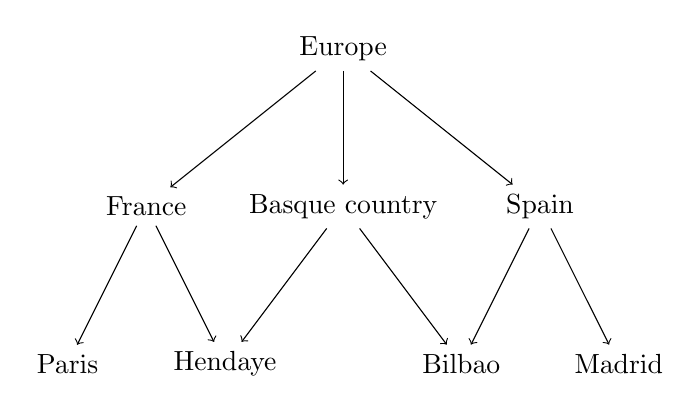
\begin{tikzpicture}
		\node[] at(1.5, 2) (E) {Europe};
		\node[] at(-1, 0) (F) {France};
		\node[] at(4, 0) (S) {Spain};
		\node[] at(-2, -2) (P) {Paris};
		\node[] at(5, -2) (M) {Madrid};
		\node[] at(1.5, 0) (BC) {Basque country};
		\node[] at(0, -2) (H) {Hendaye};
		\node[] at(3, -2) (B) {Bilbao};
		\draw[->] (F) -- (P);
		\draw[->] (F) -- (H);
		\draw[->] (S) -- (M);
		\draw[->] (E) -- (F);
		\draw[->] (E) -- (S);
		\draw[->] (E) -- (BC);
		\draw[->] (BC) -- (H);
		\draw[->] (BC) -- (B);
		\draw[->] (S) -- (B);
	\end{tikzpicture}
	\caption[]{Hasse diagram for $\lbrace \textit{Europe}, \textit{France}, \textit{Spain}, \textit{Basque country}, \textit{Paris}, \textit{Hendaye}, \textit{Bilbao}, \textit{Madrid} \rbrace$.}\label{fig5:hasse-france-spain}
\end{figure}

This Figure suggests \textit{Spain} and \textit{France} have same granularity, because they both entail \textit{Europe}, and, at a certain level of approximation, are both directly connected to Europe. Therefore, \textit{France} and \textit{Spain} can be used to generate a Qtree layer -- as done in Figure \ref{fig5:qtree-france-wh-r}, for instance. But under this definition, \textit{the Basque country} and \textit{France} also have same granularity, again, because they both entail \textit{Europe}, and, at a certain level of approximation, are both directly connected to Europe. Therefore, a Qtree like the one in Figure \ref{fig5:qtree-tentative-chd}, whose layer corresponds to the Hamblin partition induced by the set of all country-alternatives, plus the \textit{Basque country}-alternative, \textit{could} be evoked by both $S_p$ and $S_q$.\\

There remains one way to rule out that kind of Qtree, based on the independently motivated principle of Question-Cell Matching \citep{Fox2018}, given in (\ref{ex5:question-cell-matching}). This principle states that there must be a bijection between the set of pointwise exhaustified alternatives that are part of a question's denotation, and the Hamblin partition induced by such alternatives on the CS. The main purpose of this principle, is  to derive the presupposition that embedded questions must have a maximal true answer \citep{Dayal1996}.

\begin{exe}
	\ex {\textsc{\textbf{Question-Cell Matching}}. Let $Q$ be a question (a set of potentially compatible alternatives) and let $\mathfrak{P}_{Q, CS}$ be the partition induced by $Q$ on the $CS$. The following two conditions must hold:
		\begin{itemize}
			\item Cell Identification: $\forall c \in \mathfrak{P}_{Q, CS}. \ \exists p \in Q. \ CS \cap \text{exh}(Q, p) = c$;
			\item Non-Vacuity: $\forall p \in Q. \ \exists c \in \mathfrak{P}_{Q, CS}. \ CS \cap \text{exh}(Q, p) = c$ 
	\end{itemize}}\label{ex5:question-cell-matching}
\end{exe}

(\ref{ex5:question-cell-matching}) appeals to the notion of exhaustification, which is defined in (\ref{ex5:exh}). Very roughly, the exhaustification operator exh can be understood as a covert variant \textit{only}. More precisely, exh strengthens its prejacent with the negation non-weaker alternatives, in a non-arbitrary way (Innocent Exclusion, see (\ref{ex5:ie})), and also, asserts any remaining alternatives consistent with this strengthened meaning, again, in a non-arbitrary way (Innocent Inclusion, see (\ref{ex5:ii})).
\begin{exe}
	\ex {\textsc{\textbf{Exhaustification}} \citep{Fox2007,BarLev2017}. Let $p$ be a proposition and let $Q$ be a set of relevant alternatives to $p$ that are at most as complex as $p$, in the sense of \citet{Katzir2007}.\\
		The exhaustification of $p$ (prejacent) given $Q$, corresponds to $p$, conjoined with (i) the negation of all Innocently Excludable alternatives, and (ii) all Innocently Includable alternatives. In other words, exh($Q$, $p$) = $p \wedge \bigwedge_{p' \in IE(Q, p)} \neg p' \wedge \bigwedge_{p' \in II(Q, p)} p'$.}\label{ex5:exh}
	\begin{xlist}
		\ex {\textsc{\textbf{Innocent Exclusion}}. $p'$ is Innocently Excludable given $Q$ and $p$ ($p' \in IE(Q, p)$), iff $p'$ belongs to the intersection of the maximal subsets of $Q$ whose grand negation is consistent with $p$. In other words, $p' \in IE(Q, p) \iff p' \in \bigcap MaxExcl(Q, p)$, where $MaxExcl(Q, p) = Max_{\subseteq}(\lbrace Q' \subset Q. \ p \wedge \bigwedge_{p' \in Q'} \neg p' \not\vDash \bot \rbrace)$.}\label{ex5:ie}
		\ex {\textsc{\textbf{Innocent Inclusion}}. $p'$ is Innocently Includable given $Q$ and $p$ ($p' \in II(Q, p)$), iff $p'$ belongs to the intersection of the maximal subsets of $Q$ whose grand conjunction is consistent with $p$ conjoined with the negation of Innocently Excludable alternatives. In other words, $p' \in II(Q, p) \iff p' \in \bigcap MaxIncl(Q, p)$, where $MaxIncl(Q, p) = Max_{\subseteq}(\lbrace Q' \subset Q. \ p \wedge \bigwedge_{p' \in IE(Q, p)} \neg p' \wedge \bigwedge_{p' \in Q'} p' \not\vDash \bot \rbrace)$.}\label{ex5:ii}
	\end{xlist}
\end{exe}

(\ref{ex5:question-cell-matching}) was posited based on the standard semantics and pragmatics of questions, whereby questions denote sets of alternative propositions, which, at the pragmatic level, induce a partition of the CS (i.e. a depth-$1$ Qtree). But it can be naturally extended to recursive partitions, i.e. Qtrees. In Qtrees evoked by simplex sentence, each layer corresponds to the Hamblin partition induced by a set of same-granularity alternatives. So, we can reasonably assume that Question-Cell Matching, should apply to each layer of such Qtrees.

Until now, the absence or presence of this principle did not have any effect, because we only considered Qtrees generated from sets of same-granularity alternatives that were already exclusive, i.e. such that the mapping between same-granularity alternatives and partitions/Qtree layers, was always guaranteed. However, this kind of mapping is not guaranteed in the case of Figure \ref{fig5:qtree-tentative-chd}. We now show that assuming (\ref{ex5:question-cell-matching}) applies to each layer of Qtrees evoked by simplex LFs, allows to rule out the problematic Qtree in Figure \ref{fig5:qtree-tentative-chd}.

As previously observed, the unique layer of this Qtree, is generated from the set of same-granularity alternatives containing all country-alternatives, plus the \textit{Basque country} alternative. The goal is then to check if the pointwise exhaustifications of such alternatives, are in a bijective relation with the leaves of the Qtree in Figure \ref{fig5:qtree-tentative-chd}. (\ref{ex5:pointwise-exh}) computes the exhaustified counterparts of country alternatives, supplemented by the \textit{Basque country} alternative. First, let us notice that all these alternatives are logically independent; in particular, no alternative in that set is weaker than another alternative. Given this, there are three subcases to discuss: (i) the case of \textit{France}/\textit{Spain}; (ii) the case of other country alternatives like \textit{Italy}; and (iii) the case of the \textit{Basque country} alternatives. Starting with \textit{France} (or alternatively \textit{Spain}), it can be non-arbitrarily strengthened with the negation of all other alternatives. Because \textit{France} already entails the negation of all other countries, the only meaningful strengthening is the negation of \textit{the Basque country}. No alternative can be additionally asserted without contradicting this meaning, so Innocent Inclusion is vacuous. Thus, $\text{exh}(Q, \textit{France}) = \textit{France}\wedge\neg\textit{Basque}$ (see \ref{ex5:pointwise-exh-fr}). The same holds \textit{mutatis mutandis} for the \textit{Spain} alternative: $\text{exh}(Q, \textit{Spain}) = \textit{Spain}\wedge\neg\textit{Basque}$ (see (\ref{ex5:pointwise-exh-sp})). Let us now consider the case of other country alternatives, like \textit{Italy}. \textit{Italy} can be strengthened with the negation of all other alternatives in the set, but this strengthening is vacuous, because country alternatives are exclusive, and the Basque country is not in Italy. No alternative can be additionally asserted without contradicting this meaning, so Innocent Inclusion is also vacuous. Thus, $\text{exh}(Q, \textit{Italy}) = \textit{Italy}$ (see (\ref{ex5:pointwise-exh-it})), and this holds for all other country alternatives different from \textit{France} and \textit{Spain}. Lastly, turning to  the case of \textit{the Basque country}, this alternative could in principle be non-vacuously strengthened with the negation of \textit{France} (to mean \textit{the Spanish Basque country}), or, with the negation of \textit{Spain} (to mean \textit{the French Basque country}). But negating \textit{both} alternatives would lead to a contradictory meaning, and negating only one of the two, would be arbitrary. Therefore, Innocent Exclusion is vacuous. The same issue arises when considering Innocent Inclusion: \textit{the Basque country} could be non-vacuously strengthened with the assertion of \textit{France} (to mean \textit{the French Basque country}), or, with the assertion of \textit{Spain} (to mean \textit{the Spanish Basque country}). But asserting \textit{both} alternatives would lead to a contradictory meaning, and asserting only one of the two, would be arbitrary. Therefore, Innocent Inclusion is also vacuous, and $\text{exh}(Q, \textit{Basque}) = \textit{Basque}$ (see \ref{ex5:pointwise-exh-bc}).

\begin{exe}
	\ex {Pointwise exhaustification of $Q = \lbrace \textit{France}, \textit{Spain}, ..., \textit{Italy}, \textit{the Basque country}\rbrace$
	\begin{xlist}
		\ex {$\text{exh}(Q, \textit{France}) = \textit{France}\wedge\neg\textit{Basque}$}\label{ex5:pointwise-exh-fr}
		\ex {$\text{exh}(Q, \textit{Spain}) = \textit{Spain}\wedge\neg\textit{Basque}$}\label{ex5:pointwise-exh-sp}
		\ex {$\text{exh}(Q, \textit{Italy}) = \textit{Italy}$}\label{ex5:pointwise-exh-it}
		\ex {$\text{exh}(Q, \textit{Basque}) = \textit{\underline{Basque}}$}\label{ex5:pointwise-exh-bc}
	\end{xlist}}\label{ex5:pointwise-exh}
\end{exe}

Now that the relevant pointwise exhaustified same-granularity alternatives have been computed, they must be compared to the leaves of the Qtree in Figure \ref{fig5:qtree-tentative-chd}, which correspond to the cells of the Hamblin partition induced by country alternatives, plus the \textit{Basque country} alternative. This partition is summarized in (\ref{ex5:partition-countries-basque}). We then observe that there are three ``mismatches'' between the partition in (\ref{ex5:partition-countries-basque}), and the set of pointwise exhaustifications computed in (\ref{ex5:pointwise-exh}): first, the partition contains a \textit{French Basque country} and a \textit{Spanish Basque country} cell (underlined), which correspond to none of the pointwise exhaustifications in (\ref{ex5:pointwise-exh}). So the Cell Identification component of the Question-Cell Matching condition in (\ref{ex5:question-cell-matching}), is violated. Moreover, the pointwise exhaustification of \textit{the Basque country} in (\ref{ex5:pointwise-exh}), yields \textit{the Basque country} (underlined), which does not correspond to any cell in the partition in (\ref{ex5:pointwise-exh}). So, the Non-Vacuity component of (\ref{ex5:question-cell-matching}), is also violated.

\begin{exe}
	\ex {Partition induced by $Q = \lbrace \textit{France}, \textit{Spain}, ..., \textit{Italy}, \textit{the Basque country}\rbrace$ on a ``complete'' CS (equivalent to the problematic Qtree in Figure \ref{fig5:qtree-tentative-chd}):\\
		$\mathfrak{P}_{Q, CS} = \lbrace \underline{CS\wedge F\wedge B}, \underline{CS \wedge S\wedge B}, CS \wedge F\wedge \neg B, CS \wedge S\wedge \neg B, CS \wedge I, ...\rbrace$
	}\label{ex5:partition-countries-basque}
\end{exe}

Therefore, the Question-Cell Matching condition in (\ref{ex5:question-cell-matching}), is \textit{not} verified by the set of alternatives under consideration, assuming the most general CS. What about a CS which would exclude the problematic cells (underlined), i.e. would presuppose that \textit{SuB29 will not take place in the Basque country}? Such a CS would give rise to the restricted Hamblin partition in (\ref{ex5:partition-countries-basque-presupp}), for which each cell corresponds to some exhaustified alternative in (\ref{ex5:pointwise-exh}).
\begin{exe}
	\ex {Partition induced by $Q = \lbrace \textit{France}, \textit{Spain}, ..., \textit{Italy}, \textit{the Basque country}\rbrace$ on a CS entailing $\neg B$:\\
		$\mathfrak{P}_{Q, CS} = \lbrace CS \wedge F\wedge \neg B, CS \wedge S\wedge \neg B, CS \wedge I, ...\rbrace$
	}\label{ex5:partition-countries-basque-presupp}
\end{exe}

Still, an issue would remain when assuming such a CS, due to the presence of the \textit{Basque country} alternative in the alternative set. This alternative would still be (vacuously) exhaustified, however its intersection with the CS would then be empty, and by definition would not correspond to any cell of the  partition in (\ref{ex5:partition-countries-basque-presupp}). Therefore, the Non-Vacuity component of (\ref{ex5:question-cell-matching}), would still be violated.\\

This overall suggests that the set of all country alternatives, supplemented with the \textit{Basque country} alternative, induces a partition of the CS violating the Question-Cell Matching condition, no matter the CS. On that basis, and assuming that the same principle applies to the formation of layers in Qtrees evoked by simplex sentences, the Qtree depicted in Figure \ref{fig5:qtree-tentative-chd} should \textit{not} be evoked by $S_p$ or $S_q$, and, consequently, the disjunctions of $S_p$ and $S_q$, should \textit{not} evoke any well-formed Qtree. This Appendix showed that, even under a strict interpretation of what it means for two alternatives to be same-granularity, the result established in Section \ref{sec5:chds} is preserved -- assuming that the independently motivated Question-Cell Matching condition applies to Qtree formation.








